
\documentclass{LU}

\title{Digitālās aparatūras projektēšanas tiešsaistes platforma}	   
\thesistype{Bakalaura darbs}
\author{Krišjānis Veinbahs}
\studentid{kv18042}
\supervisor{prof., Dr. Dat. Leo Seļāvo}
\university{Latvijas Universitāte}
\faculty{Datorikas Fakultāte}
\location{Rīga}

% apzīmējumu saraksts
\makeglossaries

\newglossaryentry{fpga}
{
    name=FPGA,
    description={Lauka programmējamās ventiļu matricas}
}

\newglossaryentry{netlist}
{
    name=Netlist,
    description={Elektronisku elementu savienojumu apraksts jeb elektriskās ķēdes apraksts, ko atgriež HDL valodas}
}

\newglossaryentry{ttl}
{
    name=TTL,
    description={Tranzistora-tranzistora loģika}
}

\newglossaryentry{usb}
{
    name=USB,
    description={Universālā seriālā kopne}
}

\newglossaryentry{uuid}
{
    name=UUID,
    description={Vispārēji unikāls identifikators}
}

\newglossaryentry{uart}
{
    name=UART,
    description={Universālais asinhronais raiduztvērējs}
}

\newglossaryentry{fullduplex}
{
    name=Full duplex,
    description={Pilnduplekss jeb datu pārraide divos virzienos tajā pašā laikā, pretēji "pusduplekss" (angl. "half duplex")}
}

\newglossaryentry{serialport}
{
    name=Serial port,
    description={Seriālā pieslēgvieta jeb pieslēgvieta ar vienu vai diviem slēgumiem, kas nodrošina pilndupleksa 
        vai pusdupleksa datu apmaiņu}
}

\newglossaryentry{server}
{
    name=Platformas serveris,
    description={Izstrādātās platformas sastāvdaļa - serveris, kas nodrošina klientiem un aģentiem savienojumus, 
        lai realizētu centralizētu datu apmaiņu starp tiem}
}

\newglossaryentry{agent}
{
    name=Platformas aģents,
    description={Izstrādātās platformas sastāvdaļa, tipiski mikrokontrolieris, piem. Raspberry Pi, kas 
        funkcionē kā komunikācijas starpnieks starp fiziski pieslēgtu attīstītājrīku un tīklā 
        savienotu centralizētu platformas serveri}
}

\newglossaryentry{pubsub}
{
    name=Pub/Sub,
    description={Asinhrons ziņapmaiņas mehānisms, kur informācijas ražotāji publicē informāciju pēc kāda temata 
        un informācijas klausītāji abonējas šiem tematiem}
}

\newglossaryentry{client}
{
    name=Platformas klients,
    description={Izstrādātās platformas sastāvdaļa - komandrindas rīks, kas nodrošina platformas gala lietotājiem
        iespēju mijiedarboties ar platformas piedāvāto funkcionalitāti}
}

\newglossaryentry{vinterface}
{
    name=Platformas virtuālā saskarne,
    description={Izstrādātās platformas sastāvdaļa - mehānisms jeb tekstuāla vai grafiska saskarne, kas nodrošina 
        platformas lietotājam iespēju mijiedarboties ar attīstītājrīku aparatūru attālināti, imitējot klātienes 
        mijiedarbības pieredzi}
}

\newglossaryentry{mgmtpanel}
{
    name=Platformas pārvaldības panelis,
    description={Izstrādātās platformas sastāvdaļa - grafiska tīmekļa saskarne jeb mājaslapa - pārvaldības panelis, 
        kas nodrošina iespēju autentificēties un apskatīt visus platformā pieejamos statiskos datus, kā arī izveidot
        jaunus lietotājus un pārvaldīt to tiesības}
}

\newglossaryentry{actorsystem}
{
    name=Actor system,
    description={Aktieru sistēma jeb aktieru modeļa koncepts par hierarhisku informācijas sistēmu, kas sastāv no aktieriem}
}

\newglossaryentry{actor}
{
    name=Actor,
    description={Aktieru modeļa koncepts par aktieri jeb informācijas vienību, kam piemīt dzīvescikls, 
        kas var sūtīt ziņas citiem aktieriem, kas var izveidot jaunus aktierus}
}

\newglossaryentry{board}
{
    name=FPGA attīstītājrīka aparatūra,
    description={Izstrādes aparatūra, lai projektētu digitālas iekārtas}
}

\newglossaryentry{petcattle}
{
    name=Pet vs Cattle,
    description={Mājdzīvnieki vs Ganāmpulks. DevOps industrijas koncepts par pārvaldāmas aparatūras veidiem, kur
        par mājdzīvnieku tiktu uzskatīta datubāze, jo tāda parasti ir viena un par to ir ļoti jārūpējas, savukārt,
        par ganāmpulku tiktu uzskatīta slodzes balansējams tīmekļa serveru klasteris, kur jebkura servera instance
        var salūzt, bet klasteris turpinās strādāt slodzes balansēšanas dēļ}
}

\newglossaryentry{wasm}
{
    name=WASM,
    description={WebAssembly. Binārs instrukciju formāts stekā bāzētai virtuālai mašīnai}
}

\newglossaryentry{hdl}
{
    name=HDL,
    description={Aparatūras projektēšanas valoda (angl. Hardware Design Language), piemēram, Verilog un VHDL}
}

\newglossaryentry{dip}
{
    name=DIP,
    description={Digitālo Iekārtu Projektēšana. No Latvijas Universitātes Datorikas fakultātes kursa DatZ7034. 
        Alternatīva nosaukumam "Digitālās Aparatūras Projektēšana", kas izmantots platformas rīkiem}
}

\begin{document}

\maketitle

\renewcommand{\abstractname}{}
\begin{abstract}
    \begin{center}
    \Large\textbf{ANOTĀCIJA}\\
    \end{center}
    \vspace{1.5\baselineskip}

    Darba mērķis ir izstrādāt un analizēt tiešsaistes platformu digitālās aparatūras attīstītājrīku
    attālinātai pārvaldībai, programmaparatūras jeb projektējumu glabāšanai un šīs programmaparatūras testēšanai
    platformā pieejamajos attīstītājrīkos.

    Darbā tiek apskatīta platformas darbības mehānismu modelēšana, sarežģījumi šādas
    platformas izstrādē, izmantotie risinājumi un to arhitektūra.

    Precīzāk, darbā tiek apskatīta vāja reāllaika attālinātas mijiedarbības
    realizācija starp platformas lietotājiem un digitālo aparatūru, tai skaitā attālināta
    noprogrammēšana, testēšana un izmantošana. Tiek apskatītas, analizētas un
    izstrādātas arī dažādas papildus funkcionalitātes, kas uzlabo šo platformas pieredzi.

    \textbf{Atslēgas vārdi}: FPGA, UART, reāllaiks, notikumu sistēma, aktieru modelis.
\end{abstract}
 

\selectlanguage{english}
\renewcommand{\abstractname}{}
\begin{abstract}
    \begin{center}
    \Large\textbf{ABSTRACT}\\
    \Large\text{AN ONLINE PLATFORM FOR HARDWARE}\\
    \Large\text{DESIGN, ENGINEERING AND TESTING}\\
    \end{center}
    \vspace{1.5\baselineskip}

    This work contains details regarding the development and analysis of an online platform for
    managing digital hardware development boards and for managing and testing prototype firmware on these boards.

    Also this work encompasses process modelling of such a platform, complications encountered in development and
    the solutions and architecture for solving these complications.  

    More specifically this work describes a soft realtime system for remote interaction between platform users and 
    available digital hardware development boards i.e. board programming, prototype firmware testing and information exchange.
    In addition some extra features for better user experience in the platform are implemented and described.  

    \textbf{Keywords}: FPGA, UART, realtime, event system, actor model.
\end{abstract}
\selectlanguage{latvian}

\pagenumbering{gobble} 

\tableofcontents

%------------------------------------------------APZĪMĒJUMI---------------------------------------------------------

\printglossary[type=main,title={APZĪMĒJUMU SARAKSTS},toctitle={Apzīmējumu saraksts}]

\pagenumbering{arabic} % sākam numurēt lapas no apzīmējumu saraksta (3. pielikums iekš LU 03.02.2012, 1/38 ) 

\chapter*{Ievads} % * nepieliks numuru pie nosaukuma
\addcontentsline{toc}{chapter}{Ievads}
\pagestyle{plain}
Digitālās aparatūras projektēšana ir loģisku elementu konfigurāciju un
savstarpējo savienojumu plānošana, lai rezultātā aprakstītu ierīci jeb
aparatūru, kas veiktu autora jeb izstrādātāja iedomāto funkcionalitāti,
piemēram, lai izveidotu veļasmašīnas kontrolieri vai datora procesoru, vai citu
digitālās aparatūras risinājumu.  
  
Digitālās aparatūras prototipēšana ir loģisko elementu konfigurācijas sintēze,
augšupielāde un testēšana. Loģisko elementu konfigurāciju ir iespējams
augšupielādēt \gls{fpga} attīstītājrīkā, tam nolasot šo konfigurāciju un
pārkonfigurējot sevī esošo \gls{fpga} mikroshēmu, lai tā darbotos atbilstoši
dotās aparatūras aprakstam. \cite[para. II]{HerreraAlzu2013}  
  
Darba ietvaros uzmanība tiek koncentrēta uz šī digitālās aparatūras izstrādes
dzīvescikla prototipēšanas fāzi jeb brīdi, kad tiek izstrādāts
programmaparatūras prototips, tas tiek augšupielādēts attīstītājrīkā un tiek
pārbaudīta attīstītājrīka uzvedība atbilstoši vēlamajai gala aparatūras
funkcionalitātei.

Šī darba mērķis ir uzlabot šo izstrādes procesu, pārveidojot attīstītājrīku jeb
fiziskās tehnikas pārvaldību, programmēšanu un testēšanu no fiziska procesa par
digitālu procesu, izstrādājot jaunu platformu šim nolūkam. Darbā risinātā
problēma ir - vai ir iespējams virtualizēt fizisku digitālu iekārtu
projektēšanu, izstrādājot tam paredzētu tiešsaistes platformu?

Eksistē līdzīgas platformas, kas virtualizē jeb abstrahē darbu ar \gls{fpga}
ierīcēm \cite[para. I]{VaishnavAnuj2018}, taču šajā darbā izstrādātā platforma
ir īpaša ar mērķi un mērķauditoriju - attālinātas prototipēšanas darbu
nodrošināsanai studentiem. 

Jaunizveidotās platformas pielietojums, sākotnēji ir mērķēts izmantošanai
studentiem LU Digitālo Iekārtu Projektēšanas (\gls{dip}) kursā (DatZ3074
\cite{DatZ3074}), bet koncepts par šādu platformu būtu arī plašāk pielietojams
profesionālajā industrijā, ja darbā izstrādāto platformu paplašīnātu vairākiem
lietošanas mērķiem.

Darba autoritatīvs nosaukums varētu būt arī "FPGA kā pakalpojums" (angl. "FPGA
as a service"), taču šajā darbā \gls{fpga} attīstītājrīki tiek uzskatīti kā
mājdzīvnieki nevis kā ganāmpulks (angl. \gls{petcattle}), tātad
programmaparatūra tiek augšupielādēta precīzā lietotāja definētā attīstītājrīkā
nevis kādā abstraktā ierīcē, kuru platforma automātiski ieplānotu lietotāja
izmantošanai, kas ir pretēji tipiskām "X as a service" platformām.


%------------------------------------------------DARBS--------------------------------------------------------------

\chapter{Pašreizējā situācija}
\section{Problēmas pamatnostādne}

Darbā risinātā problēma ir - vai ir iespējams digitalizēt fizisku digitālu
iekārtu projektēšanu, izstrādājot tam paredzētu tiešsaistes platformu?

Darbā tiek izstrādāta šāda platforma, tiek apskatītas dažādas tehniskas
problēmas šādas platformas izstrādē un attiecīgi risinājumi šīm problēmām. 

Šī darba pirmstecī jeb kursa darbā, tika secināts, ka, lai gan eksistē dažādas
tiešsaistes platformas, lai uzturētu datu apmaiņu starp fizisku aparatūru un
platformas lietotājiem, tās pārsvarā vai nu 1) koncentrējas uz aparatūras
izejdatu monitorēšanu vai 2) uz komandu un atbilžu veida datu apmaiņu.
\cite[para. 3]{VeinbahsKrisjanis2021}

Papildus kursa darba ietvaros tika secināts, ka šo situāciju būtu iespējams
uzlabot izveidojot platformu, kas realizētu vāja reāllaika datu apmaiņu starp
aparatūru un lietotājiem, tādējādi risinot darbam aktuālo problēmu, dodot
lietotājiem iespēju mijiedarboties ar aparatūru attālināti, bet ar vienlīdz
līdzīgu sajūtu kā, ja tas notiktu fiziski, klātienē. \cite[para.
5]{VeinbahsKrisjanis2021} 

Darbs ir rakstīts kā mērķauditoriju uzskatot cilvēkus ar tehniskām iemaņām,
primāri datorinženierus, taču darbs ir sarakstīts tā, lai to varētu saprast
jebkurš datorikas students, pasniedzējs, kolēģis.

Nodaļā \ref{teorija} tiek apskatītas aktieru sistēmas un notikumu sistēmas, lai
saprastu konceptu, kas izmantots, lai realizētu vāja reāllaika komunikāciju
starp \glslink{server}{serveri}, \glslink{agent}{aģentiem} un
\glslink{client}{klientiem}. Savukārt, nodaļā \ref{risinajums} jau tiek
aprakstīta realizētā platforma, tās apakšsistēmas un rīki un darbības mehānismi.

\section{Saistība ar citiem pētījumiem}

Šis darbs ir autora kursa darba konceptuāls turpinājums. Autora kursa darbā tika veikts virspusējs problēmas
apskats par to, kas būtu nepieciešams, lai realizētu digitālu sistēmu mijiedarbībai starp fizisku digitālu 
aparatūru un sistēmas lietotājiem. Šājā darbā tiek izstrādāta konkrēta sistēma, lai panāktu digitālās aparatūras 
prototipēšanas fāzes digitalizāciju, kā arī tiek analizēti un modelēti dažādi procesi un grūtības šādas sistēmas
izstrādē. \cite{VeinbahsKrisjanis2021}



\chapter{Teorija}
\section{Aktieru modelis}

Aktieru modelis apraksta veidu kā realizēt vienotu atteikumnoturīgu informācijas
sistēmu, kas sastāv no vairākām atsevišķām, paralēli darbinātām mazākām
informācijas sistēmām - aktieriem. Aktieru modelī aktieri var 1) sūtīt ziņas, 2)
izveidot jaunus \glslink{actor}{aktierus} un 3) definēt kā reaģēt uz ziņām kas
tiek adresētas tiem pašiem. \cite[p. 1]{CarlHewitt2010}

Svarīga īpatnība aktieru modelī, kas ļauj tam labi aprakstīt reālu, fizisku
infrastruktūru (kas ir svarīgi šī darba ietvaros, jo ir nepieciešams modelēt
fizisku attīstītājrīku aparatūru), ir pamatprincips, ka aktieriem piemīt laicīgs
dzīvescikls jeb jebkurā brīdī tie var sākt darboties vai beigt darboties.
\cite[p. 6]{CarlHewitt2010} 
 
Šī īpatnība ir noderīga darba ietvaros, jo fiziskā aparatūra var salūzt, zaudēt
elektrību, zaudēt interneta savienojumu, utml. Kā arī šis modelis ir vērtīgs, jo
eksistē publiski pieejami satvari, kas ir izstrādāti pēc šī modeļa un tātad ļauj
projektēt šāda veida sistēmas. Šī darba ietvaros ir izmantots satvars Akka, kas
ir pieejams Java, Scala un .NET programmēšanas valodās, taču konceptuāli līdzīgi
satvari eksistē arī daudzās citās valodās, piem. Erlang valodā OTP satvars, Rust
valodā Actix, Haskell valodā Cloud Haskell, utml.

\begin{figure}[H]
    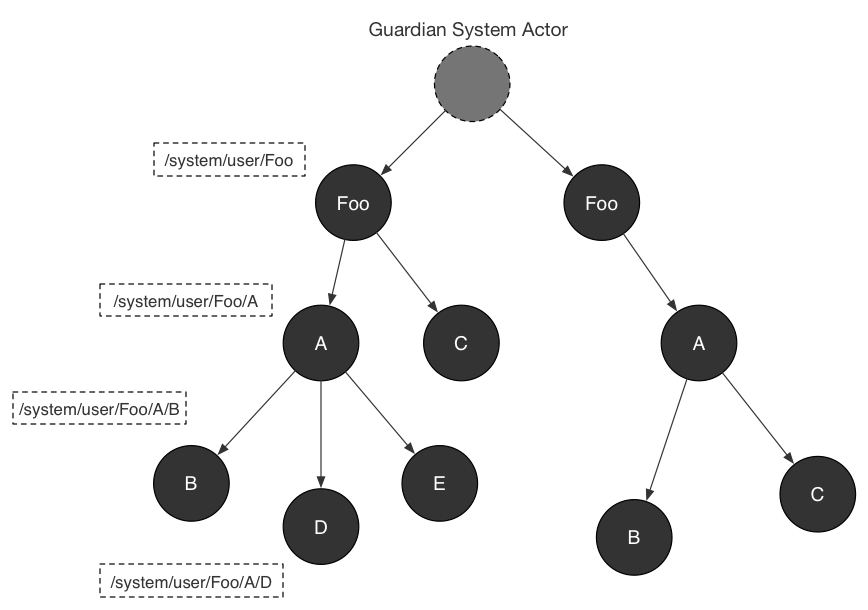
\includegraphics[width=0.5\linewidth]{assets/akka-actor-hierarchy-gray.png}
    \centering
    \caption{\glslink{actorsystem}{Aktieru modeļa sistēmas} hierarhija.
    \cite[sl. 34]{MarkusJuraAkka}}
    \label{fig:actorsystem}
\end{figure}

Attēlā \ref{fig:actorsystem} redzama aktieru modelim specifiskā aktieru sistēmas
hierarhija - kuru "bērna" aktieri izveidojis kurš "vecāka" aktieris. Aktieru
sistēmas parasti sastāv no sistēmas aktieriem un lietotāja aktieriem, parasti ir
viens saknes aizbildnības aktieris, kas izveido sistēmas un lietotāju
aizbildnības aktierus, savukārt, programmētājs izmanto šo lietotāju aizbildnības
aktieri, lai izveidotu savu biznesa loģikas saknes aktieri, kas savukārt
izveidos veselu biznesa loģikas aktieru hierarhiju atbilstoši vajadzībām.
\cite[para. The Akka actor hierarchy]{LightbendAkka2619}

\section{Notikumu sistēmas}

Piedāvātajā risinājumā caurvijas koncepts par notikumu sistēmām. Notikumu
sistēma ir tāda informācijas sistēma, kas apstrādā komandas jeb vēlamās izmaiņas
sistēmā, potenciāli akceptē komandas notikumos jeb veiktajās izmaiņās, izmaina
sistēmas stāvokli atbilstoši šiem notikumiem jeb  izmaiņām kā arī izpilda
blakusefektus jeb reakcijas atbilstoši šiem notikumiem, lai izmainītu kādas
ārējas sistēmas stāvokli.
\cite[para. 3.2.3]{JohnsenEspen2018}

Notikumu sistēmas pamatā ir notikumu dzinējs, kas realizē vēlamo sistēmas
loģiku. Šāds dzinējs, to mazliet abstrahējot, sastāv no trīs detaļām: 1)
stāvoklis jeb dati, kas tiek sākotnēji izveidoti un tad mainīti atbilstoši
notikumiem, 2) funkcija, kas lasa šobrīdējo stāvokli un validē komandas jeb
noraida tās vai akceptē tās notikumos un 3) funkcija, kas reaģē uz notikumiem
jeb attīsta aktuālo stāvokli jeb datus un izpilda notikumu blakusefektus. Attēlā
\ref{fig:eventengine} redzams šādas sistēmas dzīvescikls jeb stāvoklis,
validācijas un attīstības funkcijas un izpildītie blakusefekti.

Notikumu sistēmas iet roku rokā ar iepriekšminēto aktieru modeli. Katru aktieri
var realizēt kā notikumu sistēmu - 1) aktieris saņem ziņas no citiem aktieriem
jeb komandas jeb vēlamās izmaiņas, tās tiek validētas jeb akceptētas vai
noraidītas, 2) komandas rezultē akceptētos notikumos, 3) notikumi izmaina
aktuālo stāvokli un rezultē blakusefektos. 

\begin{figure}[H]
    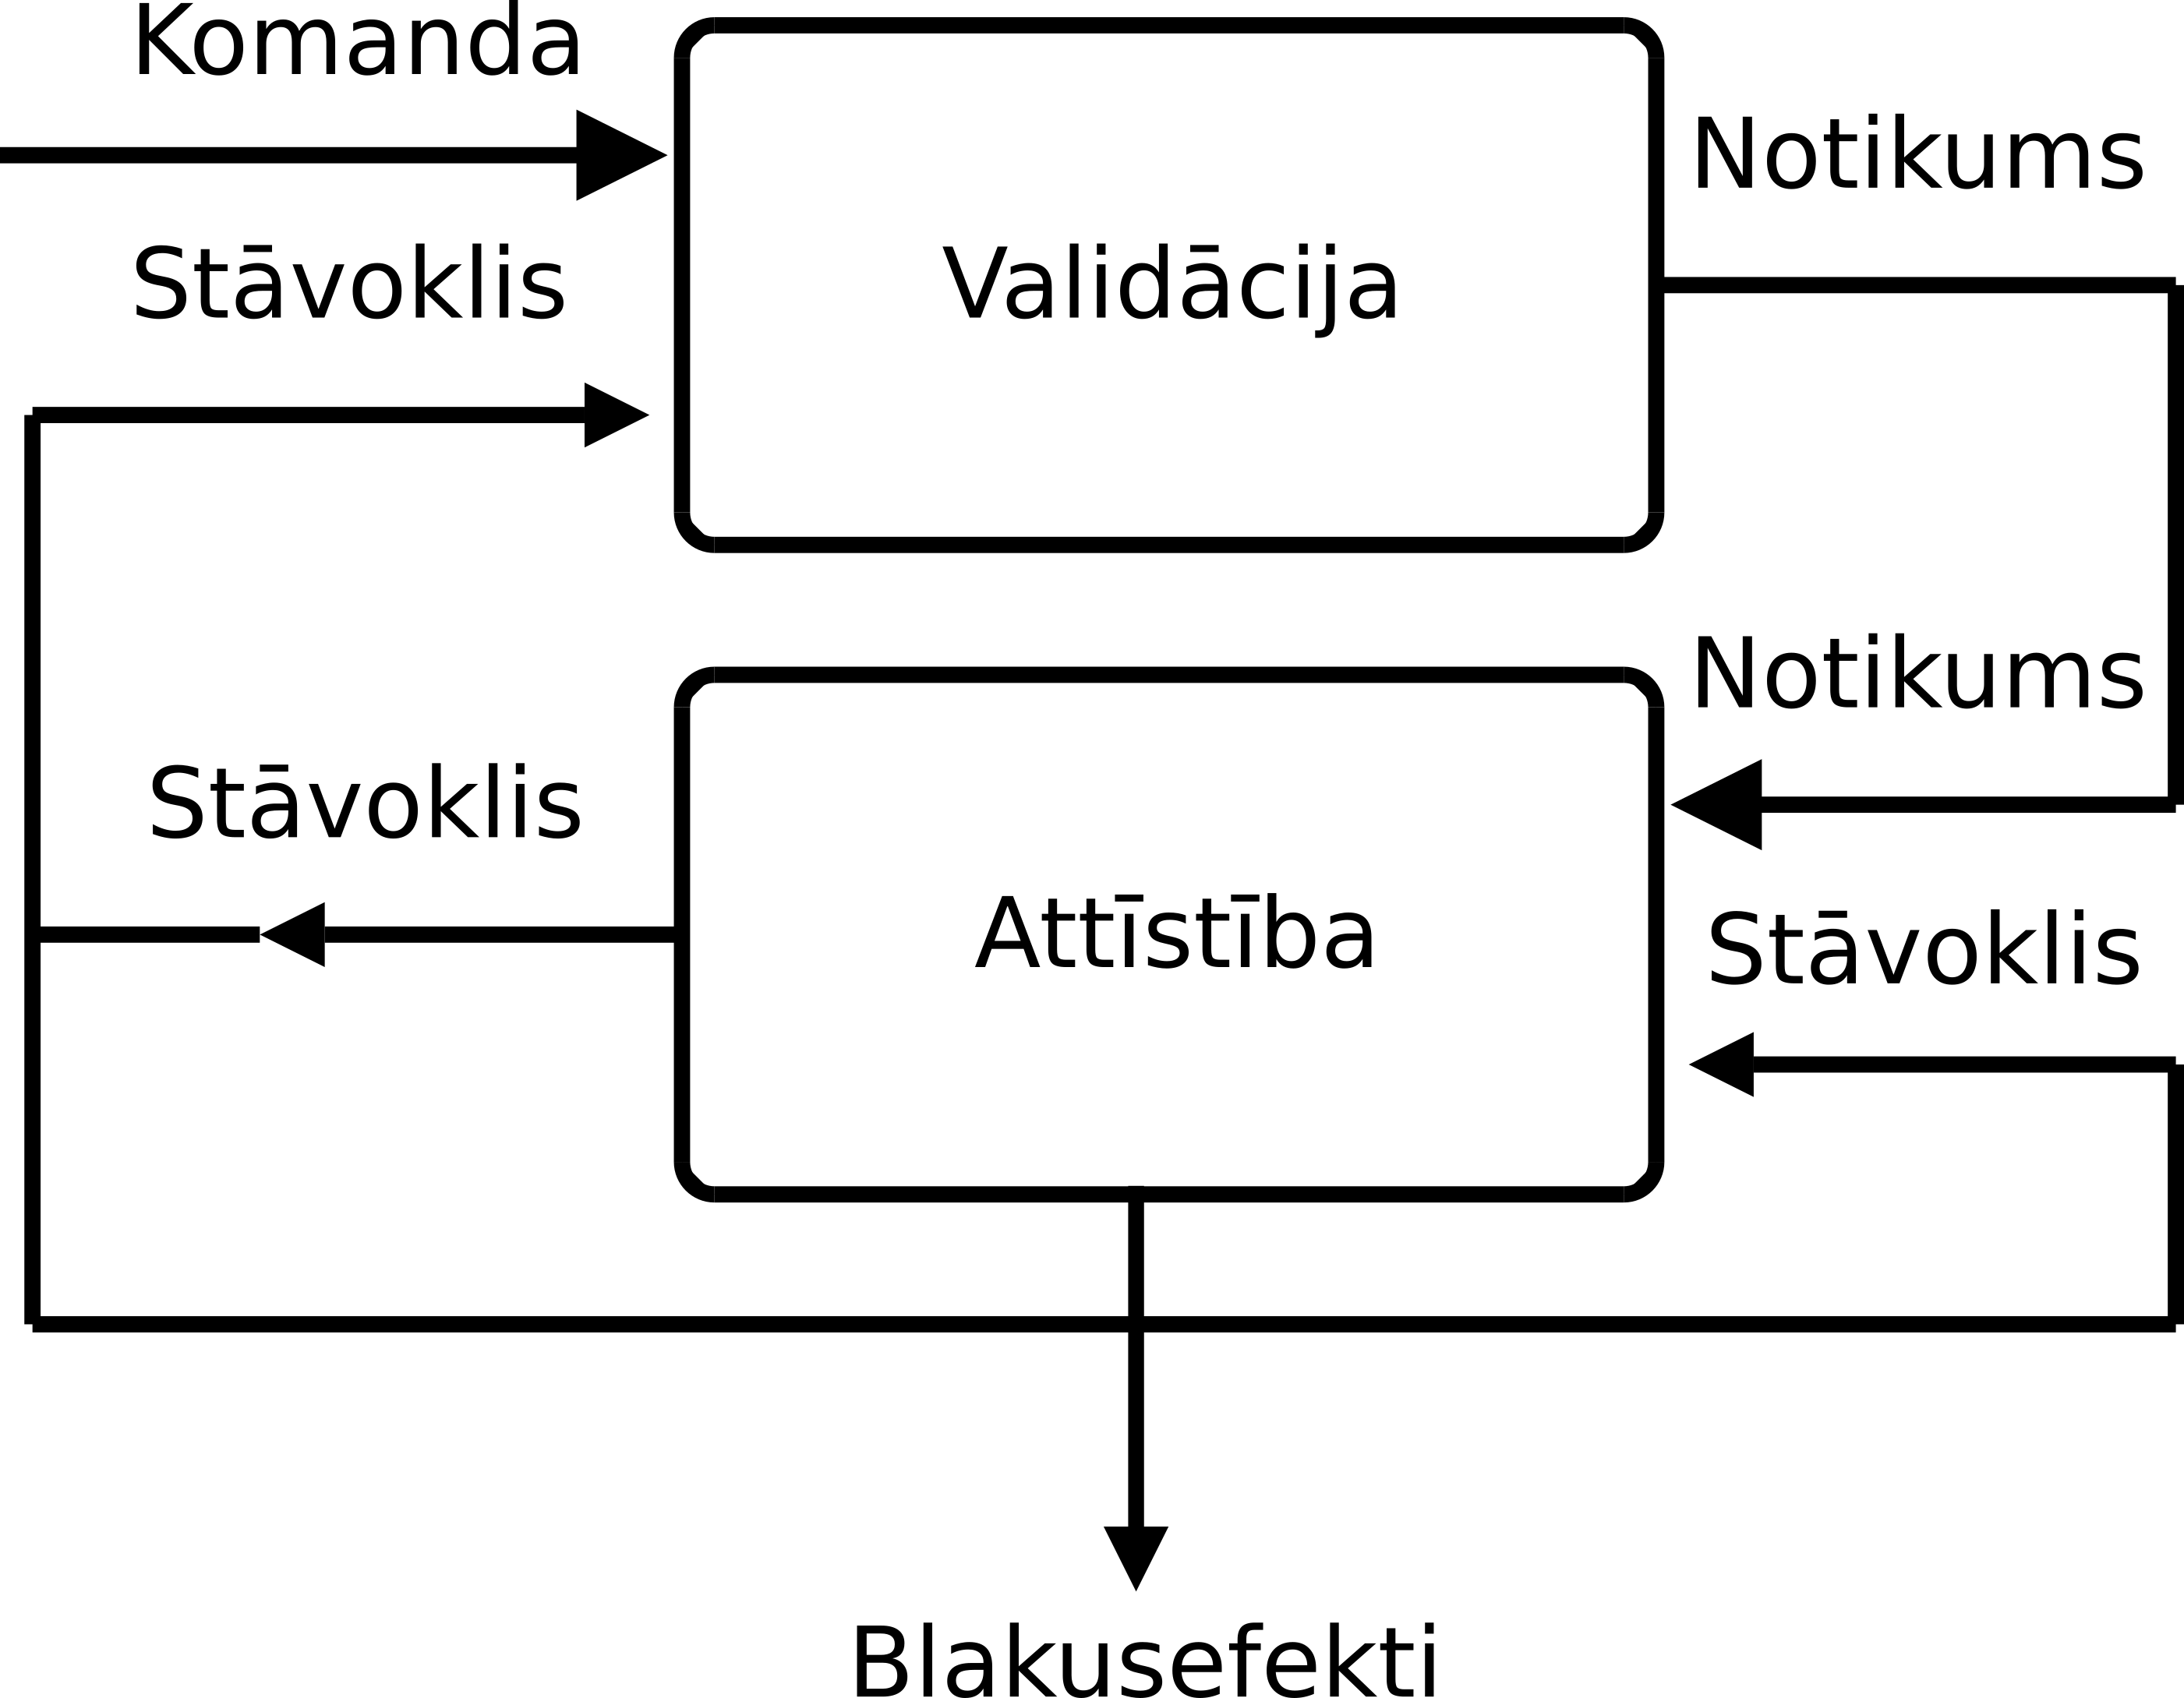
\includegraphics[width=0.5\linewidth]{assets/event-sourcing-decider.png}
    \centering
    \caption{Notikumu sistēmas apstrādes cikls. Papildināts no tiešsaistes avota. \cite{JeremieChassaing2021}}
    \label{fig:eventengine}
\end{figure}

Darba ietvaros katram attīstītājrīkam tiek piesaistīta viena vai vairākas
pārvaldības notikumu sistēmas jeb "aģenti". Aģents ir paredzēts, lai pārvaldītu
video straumēšanu, programmatūras augšupielādi, seriālā porta monitorēšanu, un
viss tiek realizēts izmantojot komandas, notikumus un blakusefektus. Tai skaitā
arī platformas lietotāji attālināti mijiedarbojoties ar attīstītājrīkiem izmanto
virtuālās saskarnes, piem. MinOS., kas arī ir realizētas kā notikumu sistēmas.
Pašā platformā, centralizētajā \glslink{server}{serverī}, lietotāju un aģentu
apkalpošanas mehānismi ir realizēti izmantojot notikumu sistēmas un aktieru
modeli. 

\section{Digitālas aparatūras projektēšana}

Lai digitalizētu mijiedarbību ar attīstītājrīku aparatūru, ir nepieciešams, lai
aparatūra ir spējīga kooperēties ar mūsu platformu, kas nozīmē, ka to ir jāprot
korekti noprogrammēt jeb, precīzāk, tajā jāaugšupielādē atbilstoši projektēta
loģisko elementu konfigurācija jeb programmaparatūra, kas nodrošinās mūsu vēlamo
mijiedarbību ar platformu.

Ir dažādi veidi kā attīstājrīka aparatūra varētu mijiedarboties ar izstrādāto
platformu, kas vēlākās nodaļās tiek arī detalizētāk apskatīti, bet pamatā ir
jāsaprot, ko īsti nozīmē digitālās aparatūras projektēšana. Digitālās aparatūras
projektēšana sevī ietver 1) signālus, 2) loģiskus elementus, 3) vadus starp tiem
loģiskajiem elementiem, 4) šo elementu izvietošanu integrētā shēmā. 

Vērtīgi pieminēt, ka loģiskie elementi šajā kontekstā nozīmē ne tikai
kombinatorās loģikas elementus, kas realizē loģikas tabulas un funkcionē bez
stāvokļa (angl. stateless), bet arī sekvenciālās loģikas elementus, kas realizē
atmiņu, piem. flip-flop. \cite[para 1.1]{LarryMassengale2018} 

\begin{figure}[H]
    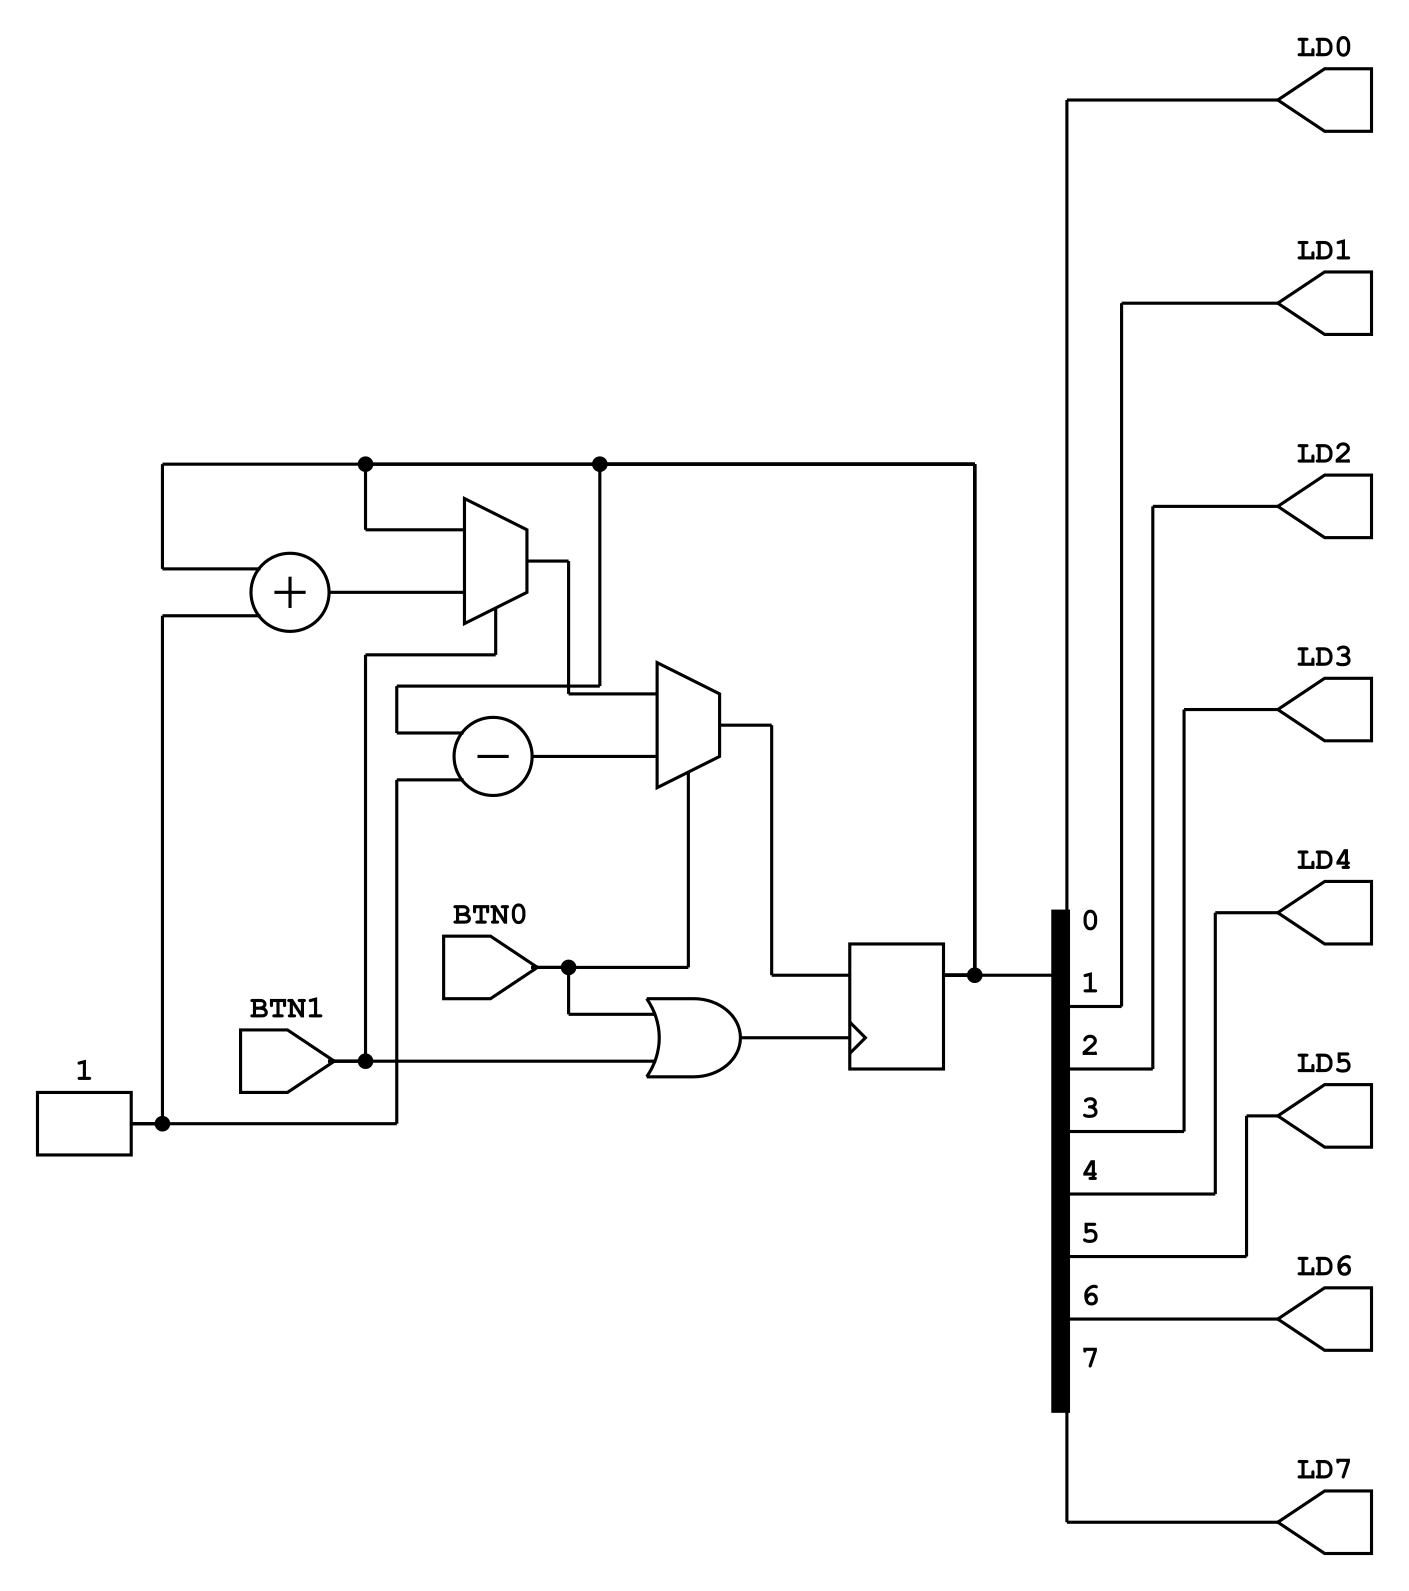
\includegraphics[width=0.5\linewidth]{assets/counter.png}
    \centering
    \caption{Loģisko elementu konfigurācija "pieskaitītājs un atņēmējs"}
    \label{fig:counter}
\end{figure}

Attēlā \ref{fig:counter} redzama tipiska loģisko elementu konfigurācija, kas
ilustrē visus iepriekšminētos projektēšanas pamatelementus. Konfigurācijā
redzami divi ievadsignāli "BTN0" un "BTN1" un astoņi "LD{0-7}" izvadsignāli.
Papildus konfigurācijā izmantots astoņu bitu atmiņas flip-flop reģistrs
(taisnstūris ar trijstūri), signālu multipleksors, kas atkarībā no "nosacījuma"
signāla ārā izvada vai nu vienu signālu vai otru (trapece), konstants astoņu
bitu signāls ar vieninieka vērtību (taisntūris ar "1"). Kad "BTN0" signāls top
no 0 par 1, reģistrā "1" tiek atņemts vieninieks. Kad "BTN1" signāls top no 0
par 1, reģistrā "0" tiek pieskaitīts vieninieks. Astoņu bitu reģistra "1" bitu
vērtība tiek izvadīta izvadsignālos "LD{0-7}". Vērts pieminēt, ka "+" un "-"
šajā ilustrācijā ir abstrakcijas, ar kurām patiesībā domāti elementi 1) astoņu
bitu "full adder" un 2) astoņu bitu "full subtractor".

Šī ilustrācija ir izveidota izmantojot "yosys" un "netlistsvg" atvērtos rīkus.
Šīs digitālās aparatūras Verilog projekta avota kods un ilustrācijas kods ir
pieejams šī projekta avota koda repozitorijā. \cite{VeinbahsKrisjanisTestbed}
Papildus tas ir pieejams arī pielikumā \ref{att:counter}.

\section{Seriālā komunikācija}

Pieņemot, ka ir iespējama centralizēta platforma, kas aprakstīta vēlākās
nodaļās, kas nodrošina datu apmaiņu starp lietotājiem un aparatūru, ir jāņem
vērā, ka, projektējot elektroniku, tomēr ir ļoti skaidri jādefinē, ko īsti
nozīmē datu apmaiņa ar aparatūru.

Šī darba ietvaros datu apmaiņa ar attīstājrīku aparatūru ir realizēta izmantojot
\glslink{serialport}{seriālo komunikāciju}. Precīzāk, \gls{fpga} tiek
augšupielādēta programmaparatūra, lai seriāli komunicētu ar attīstītājrīkā esošu
\gls{uart} kontrolieri ar diviem "RX" un "TX" signāliem, savukārt,
\gls{uart} kontrolieris šo visu pārraida pāri \gls{usb} savienojumam
\cite[para. USB-UART Bridge]{DigilentAnvylReference}, un šos datus saņem
attīstītājrīkam ar \gls{usb} vadu pievienots mikrokontrolieris, kas satur
platformas programmatūru, ko savukārt sauc par "\glslink{agent}{aģentu}". Šo
mehānismu ar \gls{ttl}, \gls{usb}, \gls{uart} komunikāciju var
apskatīt attēlā \ref{fig:agentcomms}.


\begin{figure}[H]
    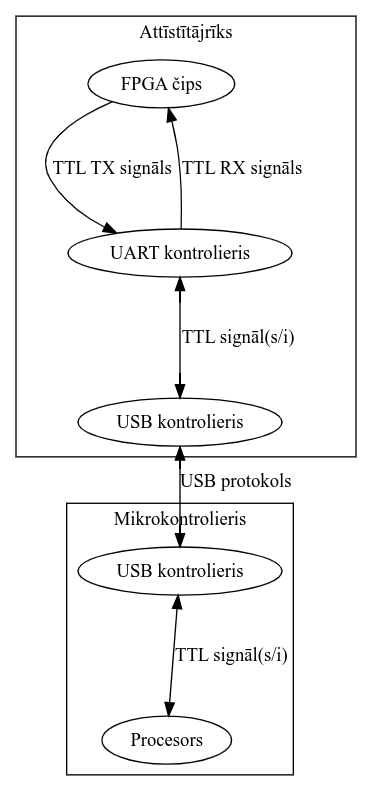
\includegraphics[width=0.3\linewidth]{assets/agentcomms-grey.png}
    \centering
    \caption{Datu apmaiņa starp attīstītājrīku un platformas "\glslink{agent}{aģentu}"}
    \label{fig:agentcomms}
\end{figure}

Ņemot vērā, šo attīstītājrīkā pieņemto komunikācijas modeli, vienīgais, ko
atliek realizēt pašam, ir projektēt \gls{ttl} seriālo komunikāciju, izmantojot
\gls{uart} mehānismu, lai nodrošinātu baitu apmaiņu starp ierīcēm. Attēlā
\ref{fig:serialframe} redzams seriālās komunikācijas kadrs iekodēts spriegumā,
ko attiecīgi var jau noprojektēt Verilog valodā, tādējādi nodrošinot
\glslink{fullduplex}{pilndupleksa} \gls{uart} baitu datu apmaiņu starp ierīcēm.
Šī darba ietvaros tika izmantota seriālā komunikācija "8-N-1" jeb ar 8 datu
bitiem, bez paritātes bita un ar vienu "stop" bitu.

\begin{figure}[H]
    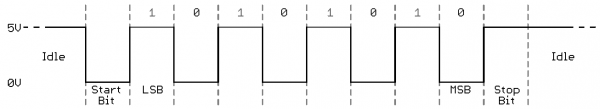
\includegraphics[width=0.7\linewidth]{assets/ttl-serial-gray.png}
    \centering
    \caption{Seriālās komunikācijas kadrs iekodēts fiziskā signālā}
    \label{fig:serialframe}
\end{figure}


\chapter{Risinājums}
\section{Digitālās aparatūras prototipēšanas platforma}
\label{sec:dipplatform}

Izstrādātā platforma sastāv no \glslink{server}{servera},
\glslink{agent}{aģentiem} jeb \glslink{board}{aparatūras} starpniekiem, pašas
fiziskās attīstītājrīku \glslink{board}{aparatūras}, \glslink{client}{klientiem}
jeb gala lietotājiem ar komandrindas rīkiem, un pārvaldības paneļa jeb datu
pārvaldības tīmekļa lietotnes. Attēlā \ref{fig:dipdpd0} redzama 0. līm. datu
plūsmas diagramma minētai platformai. 

\begin{figure}[H]
    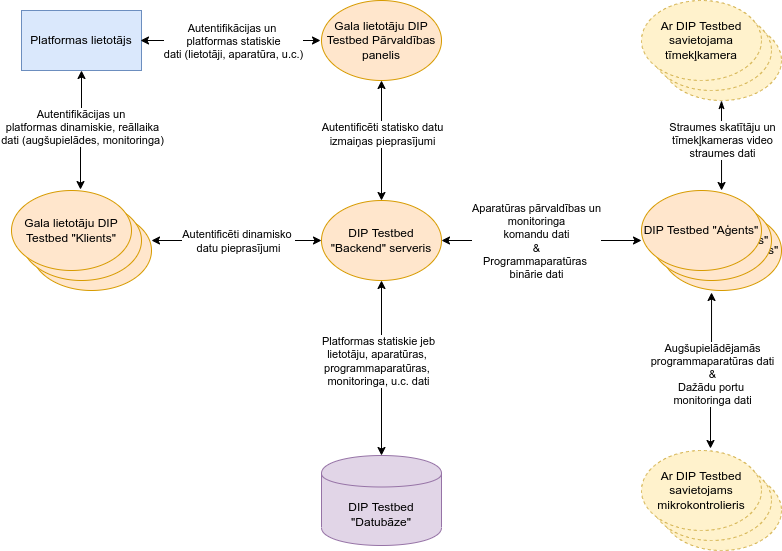
\includegraphics[width=1.0\linewidth]{assets/DPD0.drawio.png}
    \centering
    \caption{Digitālās aparatūras prototipēšanas platformas virspusēja datu plūsmas diagramma}
    \label{fig:dipdpd0}
\end{figure}

Attēlā \ref{fig:dipdpd0} redzamās apakšsistēmas ir aprakstītas šajā dokumentā
sekojoši. 

Pašā platformas centrā ir centralizēts tīmekļa \glslink{server}{serveris}, kas
funkcionē kā pārvaldības datu avots un platformas lietotāju komunikācijas
starpnieks, tā datu pārvaldības ir aprakstīta nodaļās \ref{sec:usermgmt} un
\ref{sec:hwmgmt}, savukārt, tā dalība komunikācijas mehānismos ir aprakstīta
\ref{sec:dipactorsystem}.

Nodaļā \ref{sec:dipactorsystem} aprakstītā vājo reāllaika komunikācijas sistēmu,
savukārt, izmanto komandrindas rīki - klients un aģents - lai ļautu lietotājiem
mijiedarboties ar attīstītājrīku \glslink{board}{aparatūru}. Šis mehānisms ir
aprakstīts nodaļā \ref{sec:hwmgmt}. Un izmantojot šo klienta - aģenta mehānismu,
platformā lietotājam tiek realizētas trīs \glslink{vinterface}{saskarnes}, lai
mijiedarbotos ar attīstītājrīku \glslink{board}{aparatūru}, kuras aprakstītas
nodaļās \ref{sec:vinweb}, \ref{sec:vinbytes} un \ref{sec:vinminos}.

Par šīs platformas, tai skaitā \glslink{board}{aparatūras} laboratoriju,
uzstādīšanu un administrēšanu ir aprakstīts nodaļā \ref{sec:ops}. Par
\glslink{firmware}{programmaparatūras} izstrādi un testēšanu platformā
aprakstīts nodaļā \ref{sec:maintenance}. Par šī darba veikumu un tvērumu
aprakstīts nākamajā nodaļā \ref{sec:scope}.

\section{Darba tvērums}
\label{sec:scope}

Darba ietvaros tika izstrādāta vāja reāllaika komunikācijas platforma, kas
nodrošina 1) iespēju reģistrēt un uzskaitīt, pārvaldīt \glslink{board}{fizisku
attīstītājrīku} vai mikrokontrolieru aparatūru, 2) veikt
\glslink{firmware}{programmaparatūras} augšupielādi aparatūrā, 3) mijiedarboties
ar aparatūru, izmantojot vizuālu saskarni, kas līdzinās noklusētajai aparatūrā
fiziski pieejamajai \glslink{vinterface}{saskarnei}, 4) ierobežoti testēt
aparatūras funkcionalitāti. Papildus platforma tika arī testēšanas nolūkiem
izveidota publiskā mākoņpakalpojumu serverī, kas aprakstīts avota koda
repozitorijā un nodaļā \ref{sec:ops}. \cite{VeinbahsKrisjanisTestbed}
\cite{VeinbahsKrisjanisProduction}

Šis darbs izstrādāts atvērti - platformas pirmkods un šī dokumenta pirmkods ir
publiski pieejams GitHub platformā brīvai apskatei un izmantošanai.
\cite{VeinbahsKrisjanisTestbed} \cite{VeinbahsKrisjanisThesis}.

\begin{table}[H]
    \begin{tabular}{ |p{3cm}|p{3cm}|p{3cm}|p{3cm}| }
    \hline
    Programmēšanas valoda & Faili & Komentāru rindiņas & Koda rindiņas \\
    \hline
    Python          & 101   & 717   & 7424  \\
    Scala           & 101   & 120   & 4088  \\
    Verilog         & 34    & 676   & 2496  \\
    HTML            & 11    & 0     & 492   \\
    Bourne Shell    & 17    & 85    & 378   \\
    make            & 2     & 30    & 80    \\
    SQL             & 2     & 28    & 70    \\
    XML             & 1     & 8     & 40    \\
    YAML            & 2     & 1     & 33    \\
    C++             & 1     & 14    & 14    \\
    \hhline{|=|=|=|=|}
    Kopā & 272 & 1679 & 15115\\
    \hline
    \end{tabular}
    \centering
    \captionsetup{justification=centering}
    \caption{Koda rindiņu skaita analīze projekta pirmkodā ar atvērtā koda rīku \lstinline!cloc!}
    \label{table:cloc}
\end{table}

Aptuvenai sapratnei par izstrādāto koda apjomu, projekta pirmkodā tika izpildīts
koda rindiņu analīzes rīks \cite{AlDanialCloc}, kura rezultāti redzami gan projekta
pirmkoda versiju kontroles repozitorijā \cite{VeinbahsKrisjanisTestbed}, gan tabulā
\ref{table:cloc}.

Platformas pamata funkcionalitāte, lai lietotājs augšupielādētu
\glslink{firmware}{programmaparatūru} un veiktu baitu līmeņa datu apmaiņu ar
\glslink{board}{aparatūru}, tika realizēta kursa darba laikā.

Bakalaura darba laikā, 1) platformai tika pievienota autentifikācija, 2)
izstrādāts \glslink{mgmtpanel}{pārvaldības panelis}, 3) pārrakstīts klients no
tīras grafiskas saskarnes par termināļa grafisko saskarni, 4) pārrakstīta
klienta virtuālā \glslink{vinterface}{saskarne} kā notikumu sistēma nevis
nestrukturizēts kods, 5) izplānota un realizēta virtuālā
\glslink{vinterface}{saskarne} MinOS formālā protokolā, klientā un
attīstītājrīkā, 6) tika dokumentēta sistēmas darbība un arhitektūra, tai skaitā
arī šī dokumenta izstrāde.

\section{Datu relācijas modelis}
\label{sec:staticdata}

Šī platforma pamatā sastāv no reāllaika datu starpniecības un statisku datu
pārvaldības. Par statiskajiem datiem tiek uzskatīti tādi dati, kurus lietotājs
nemaina izmantojot vājā reāllaika komunikācijas kanālus, kas aprakstīti sadaļā
\ref{sec:dipactorsystem}. 

\begin{figure}[H]
    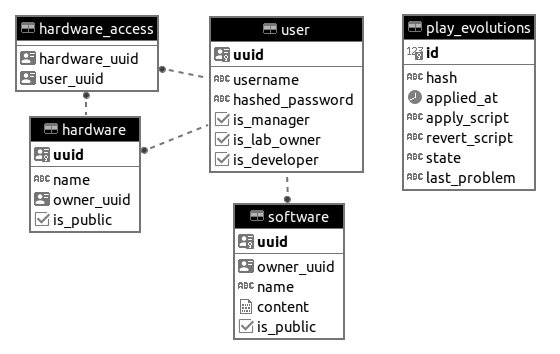
\includegraphics[width=0.7\linewidth]{assets/physical-er-diagram-gray.png}
    \centering
    \caption{Platformas fiziskā līmeņa datubāzes relāciju diagramma.}
    \label{fig:staticdata}
\end{figure}

Attēlā \ref{fig:staticdata} redzama platformas izstrādes laikā izveidotā
datubāzes fiziskā līmeņa relāciju diagramma, kurā redzamas tabulas lietotājiem
\lstinline!user!, \glslink{firmware}{programmaparatūrai} \lstinline!software!,
aparatūrai \lstinline!hardware! un \glslink{board}{aparatūras} piekļuvei
\lstinline!hardware_access!, kā arī papildus tabula datubāzes migrāciju vēstures
pārvaldībai \lstinline!play_evolutions!, kas ir noklusēts tabulas nosaukums
projektā izmantotajam Scala programmēšanas valodas tīmekļa lapu izstrādes
ietvaram "Play Framework".

Lielākoties visām biznesa loģikas entītijām ir piesaistīts \gls{uuid}
identifikators \lstinline!uuid! un nosaukums \lstinline!name!, papildus dažām
entītijām ir dažādi piekļuves dati formātā \lstinline!is_*!,
\glslink{firmware}{programmaparatūrai} ir arī tās saturs \lstinline!content! un
lietotājam ir paroles ar jaucējvērtību datiem \lstinline!hashed_password!.

\glslink{firmware}{Programmaparatūras} tabulu varētu arī saukt
\lstinline!firmware!, taču platformas izstrādes laikā tika eksperimentēts
platformā arī reģistrēt ne tikai attīstītājrīku \glslink{board}{aparatūru}, bet
arī programmējamus mikrokontrolierus, kuros augšupielādē programmatūru.

Darba ietvaros tika arī apsvērta tabula \lstinline!hardware_messages!, lai
glabātu vēsturi par notikušo vājā reāllaika komunikāciju, taču laika
ierobežojumu dēļ šī funkcionalitāte netika realizēta, jo nebija kritiska
platformas funkcionētspējai.

\section{Lietotāju datu pārvaldība}
\label{sec:usermgmt}

Lietotāju uzskaitei izmantota attēlā \ref{fig:staticdata} redzamā tabula
\lstinline!user!. Lietotājam ir iespējamas trīs iespējamas lomas pārvaldnieks
\lstinline!manager!, laboratorijas īpašnieks \lstinline!lab_owner! un
izstrādātājs \lstinline!developer!, atkarībā no kuras lietotājam platforma
piedēvē attiecīgas tiesības veikt dažādas darbības, kuras skatāmas tabulā
\ref{table:permissions}.

\begin{table}[H]
    \newcounter{permissioncounter}
    \newcommand\rownumber{\stepcounter{permissioncounter}\arabic{permissioncounter}.}
    \begin{tabular}{ |p{1cm}|p{5cm}|p{3cm}|p{6cm}| }
    \hline
    N.p.k.&Darbība&Nepieciešamās tiesības&Papildus nosacījumi \\
    \hline
    \rownumber & Lietotāja bez tiesībām izveide & - & Lietotājvārds nevar būt aizņemts \\
    \hline
    \rownumber & Lietotāju datu uzskaite & \lstinline!is_manager! vai \lstinline!is_lab_owner! & Jebkurš var lasīt savus datus \\
    \hline
    \rownumber & Lietotāja tiesību maiņa & \lstinline!is_manager! & - \\
    \hline
    \rownumber & Programmaparatūras augšupielāde & \lstinline!is_developer! & - \\
    \hline
    \rownumber & Programmaparatūras piekļuve & \lstinline!is_developer! vai
        \lstinline!is_manager! & Jebkurš var lasīt savu vai publicētu
        (\lstinline!is_public!) programmaparatūru \\
    \hline
    \rownumber & Programmaparatūras publicēšana & \lstinline!is_manager! & - \\
    \hline
    \rownumber & Aparatūras izveide & \lstinline!is_lab_owner! & - \\
    \hline
    \rownumber & Aparatūras publicēšana & \lstinline!is_manager! vai
        \lstinline!is_lab_owner! & Pārvaldnieks var publicēt visu, citi tikai
        savu \\
    \hline
    \rownumber & Aparatūras uzskaite & \lstinline!is_manager! vai
        \lstinline!is_developer!, vai \lstinline!is_lab_owner! & Pārvaldnieks
        var uzskaitīt visu, citi tikai savu vai \lstinline!hardware_access!
        tabulā piesaistīto \\
    \hline
    \rownumber & Aparatūras tiesību maiņa & \lstinline!is_manager! vai
        \lstinline!is_developer!, vai \lstinline!is_lab_owner! & Pārvaldnieks
        var pārvaldīt visu, citi tikai savu \\
    \hline
    \end{tabular}
    \centering
    \captionsetup{justification=centering}
    \caption{Lietotāju tiesības un pieejamās darbības}
    \label{table:permissions}
\end{table}

Platformā projekta \glslink{software}{programmatūras} konfigurācijā ir
konfigurējams administratora lietotājs ar visām trīs iepriekšminētajām tiesībām,
lai izveidotu sākotnējos pārvaldības lietotājus.

Platformā lietotājus un to piekļuves datus var konfigurēt no
\glslink{mgmtpanel}{pārvaldības paneļa}, kas ir atšķirīgi no pārējām platformas
darbībām, kas lielākoties norit komandu rindā jeb terminālī, jo šos datus
pārsvarā pārvalda pasniedzējs vai laboratorijas īpašnieks, kuram visvieglāk būtu
no jebkura datora atvērt pārlūku un veikt šīs darbības. Savukārt, izstrādātājam,
kas pārsvarā savu darbu veic komandurindā, lielākā daļa darbības ir pieejamas
izmantojot komandu rindas rīku jeb \glslink{client}{klientu}. Skats no
pārvaldības paneļa lietotāju sadaļas skatāms attēlā \ref{fig:mgmtpanelusr}.

\begin{figure}[H]
    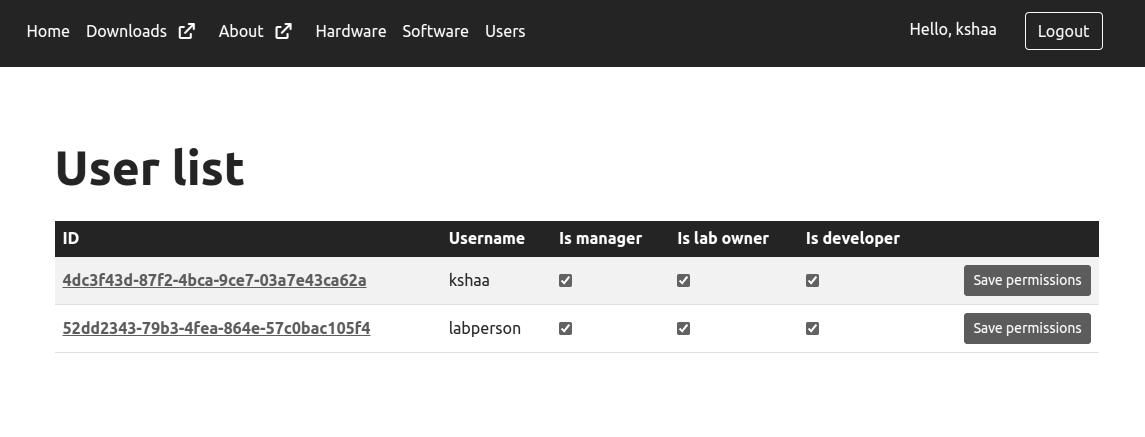
\includegraphics[width=0.9\linewidth]{assets/mgmt-panel-usr-gray.png}
    \centering
    \caption{Platformas pārvaldības paneļa lietotāju pārvaldības skats.}
    \label{fig:mgmtpanelusr}
\end{figure}

\section{Notikumu sistēmu realizācija}
\label{sec:dipactorsystem}

Darbā izstrādātajā platformā, lai veiktu ziņu starpniecību starp lietotāju un
\glslink{board}{aparatūru}, bija nepieciešams realizēt vāja reāllaika
komunikāciju. Tā ir nepieciešama, piemēram, lai sūtītu "LED gaismu" aktuālo
stāvokli no \glslink{board}{aparatūras} lietotājam un "spiedpogu" aktuālo
stāvokli no lietotāja \glslink{board}{aparatūrai} jeb lai realizētu
\glslink{vinterface}{virtuālas saskarnes}.

Lai realizētu šādu vāja reāllaika komunikācijas sistēmu, platforma tika pamatā
izstrādāta kā notikumu sistēma, izmantojot Scala programmēšanas valodas
\glslink{actor}{aktieru} modeļa programmēšanas ietvaru Akka.
\glslink{actor}{Aktieru} modelī bāzētas notikumu sistēmas ir pierādījušas sevi
kā spējīgas nodrošināt veiktspēju augstas paralelitātes reāllaika sistēmām,
piemēram, Microsoft ir izstrādājuši \glslink{actor}{aktieru} modelī bāzētu
mākoņpakalpojumu risinājumu satvaru Orleans, ar kuru tie spēja realizēt
gājienos-bāzētu spēli "Galactic Reign", kuru tie testēja ar 1000 paralēli
darbojošamies \glslink{actor}{aktieriem}, novērojot stabilu veiktspēju ar
95-97\% procesoru nodarbinātību. \cite[para. 5.1, 5.2]{Bernstein2014}.

Platformas notikumu sistēmas realizācijai pamatā ir nodaļās \ref{sec:actormodel}
un \ref{sec:eventsourcing} pieminētais \glslink{actor}{aktieru} modelis un
notikumu sistēmas.

Starp \glslink{server}{centralizēto serveri} un \glslink{client}{klientu}, un
\glslink{agent}{aģentu} komunikācija notiek, izmantojot, WebSocket un HTTP
savienojumus. WebSocket savienojumos tiek raidītas gan bināra, gan teksta
formāta ziņas, papildus šādiem savienojumiem tika realizēts, ka pirmai ziņai
vienmēr ir jābūt autentifikācijas ziņai JSON formātā, kas satur lietotājvārdu un
paroli, kā arī tika realizēts, ka ik pēc nokonfigurējama intervāla, kas pēc
noklusējuma bija 30 sekundes, klientam vai aģentam ir jāsūta sirdspuksta (angl.
heartbeat) ziņa, kas, ja netika saņemta 3 reizes pēc kārtas, ļāva secināt, ka
savienojums ir bojāts un to var izbeigt. HTTP savienojumiem autentifikācija tika
realizēta izmantojot HTTP sīkdatnes un HTTP "basic auth" galveni, papildus HTTP
savienojumu gadījumā reāllaika komunikācijas vajadzībām, tika pieņemta
konfigurējama noildze, kas pēc noklusējuma bija 30 sekundes.

Starp \glslink{board}{aparatūru} un \glslink{agent}{aģentu} ir izmantota sadaļā
\ref{sec:serial} aprakstītā seriālā komunikācija. Aģenti, kas realizēti Python
valodā izmantojot daudz dažādas publiski pieejamas bibliotēkas, ik pēc 0.01
sekundes nolasa Linux čaulas seriālo ierīču dziņu buferos ielasītos datus un tos
izsūta kā ziņu WebSocket savienojumā ar \glslink{server}{serveri}. Dati atkarībā
no aģenta veida tiek lasīti pēc dažāda "baudrate", kas pēc noklusējuma ir
115200, kas ir ātrākais Digilent Anvyl datu pārraides ātrums. Kad aģenta
\glslink{board}{aparatūras} datu ziņas tiek nosūtītas \glslink{server}{serverī},
tās tiek translētas visiem ierīces seriālā porta abonentiem Akka jeb platformas
\glslink{actor}{aktieru} klasterī, kas precīzāk aprakstīts sadaļā
\ref{sec:hwmgmt}.

Tabulā \ref{table:serveractors} ir aprakstīti platformas izstrādes gaitā
realizētie \glslink{server}{serverī} esošie \glslink{actor}{aktieri}, to
funkcija jeb biznesa loģika. Ir vērts minēt, ka šajā sarakstā nav dažādi Akka
vai Play satvaru sistēmas \glslink{actor}{aktieri}.

Tabulā \ref{table:cliactors} ir aprakstīti platformas izstrādes gaitā realizētie
aģentā un klientā realizētie \glslink{actor}{aktieri} un to apraksts. Šie
\glslink{actor}{aktieri} ir sarakstīti kopā, jo reāli tiem pamatā ir tā pati
arhitektūra, jo gan klients, gan aģents abi realizēti vienā Python koda bāzē.

\begin{table}[H]
    \newcounter{serveractorcounter}
    \newcommand\rownumber{\stepcounter{serveractorcounter}\arabic{serveractorcounter}.}
    \begin{tabular}{ |p{1cm}|p{5cm}|p{9cm}| }
    \hline
    N.p.k.&Aktieris&Aktiera funkcija \\
    \hline
    \rownumber & Abonamenti (oriģ. PubSub) & Uzskaita tematus, tā abonentus,
        saņem ziņas, publicē abonentiem \\
    \hline
    \rownumber & Vaicājumi (oriģ. Query) & Palīgaktieris, lai HTTP pieprasījumos
        izveidotu šo aktieri, izsūtītu kādu ziņu, saņemtu atpakaļ ziņu un beigtu
        darbību, kas ir noderīgi, lai integrētu HTTP saskarnes aktieru modelī \\
    \hline
    \rownumber & Tīmekļkamera (oriģ. Camera) & Saņem tīmekļa kameras datus no
        aparatūras un publicē tos tīmekļkameras abonentiem \\
    \hline
    \rownumber & Tīmekļkameras abonents (oriģ. CameraListener) & Klausās
        publicētos tīmekļa kameras datus un pāradresē tos tos tīmekļkameras
        skatītājam HTTP savienojumā kā \lstinline!application/ogg! straumi \\
    \hline
    \rownumber & Aparatūras kontrolieris (oriģ. HardwareControl) & Uztur
        WebSocket savienojumu ar aparatūru, saņem un pāradresē komandas
        aparatūrai, veic seriālās komunikācijas datu starpniecību starp
        aparatūru un aparatūras abonentiem \\
    \hline
    \rownumber & Aparatūras abonents (oriģ. SerialListener) & Uztur WebSocket
        savienojumu ar lietotāju, veic seriālās komunikācijas datu starpniecību
        starp aparatūru un lietotāju \\
    \hline
    \end{tabular}
    \centering
    \captionsetup{justification=centering}
    \caption{Platformas servera aktieri}
    \label{table:serveractors}
\end{table}

\begin{table}[H]
    \newcounter{cliactorcounter}
    \newcommand\rownumber{\stepcounter{cliactorcounter}\arabic{cliactorcounter}.}
    \begin{tabular}{ |p{1cm}|p{5cm}|p{9cm}| }
    \hline
    N.p.k.&Aktieris&Aktiera funkcija \\
    \hline
    \rownumber & Aparatūra (oriģ. Hardware) & Uztur savienojumu ar
        \glslink{server}{serveri} un aparatūru, gaida \glslink{server}{servera}
        komandas, programmē aparatūru, veic seriālo datu komunikāciju starp
        aparatūru un \glslink{server}{serveri}, ir trīs paveidi
        \lstinline!Anvyl! \gls{fpga} attīstīrājrīkam, \lstinline!nrf52!
        mikrokontrolierim un \lstinline!fake! testēšanai \\
    \hline
    \rownumber & Tīmekļkamera (oriģ. Camera) & Uztur savienojumu ar
        \glslink{server}{serveri} un tīmekļkameru, kas fiziski pievienota un
        pieejama aģenta sistēmā, sūta tīmekļkameras datus uz
        \glslink{server}{serveri} \\
    \hline
    \rownumber & Aparatūras abonents (oriģ. SerialListener) & Uztur WebSocket
        savienojumu ar lietotāju, veic seriālās komunikācijas datu starpniecību
        starp lietotāju un \glslink{server}{serveri} \\
    \hline
    \end{tabular}
    \centering
    \captionsetup{justification=centering}
    \caption{Aģentu un klientu aktieri}
    \label{table:cliactors}
\end{table}

\section{Aparatūras pārvaldība}
\label{sec:hwmgmt}

Iepriekšējās nodaļās ir aprakstīta platformas datu pārvaldība un
\glslink{actor}{aktieru} hierarhija, šī nodaļa apraksta kā šī arhitektūra
sasaistas kopā, lai realizētu digitāli pārvaldāmu \glslink{board}{FPGA
attīstītājrīku aparatūru}.

Attēlā \ref{fig:labsetup} aprakstīts kā izskatītos platformas sākotnēja
uzstādīšana, lai digitalizētu jeb padarītu pieejamu tiešsaistē laboratorijā
pieejamo \glslink{board}{aparatūru}. Tiek pieņemts, ka katrs
\glslink{server}{servera} pieprasījums rezultē veiksmīgā atbildē.

\begin{figure}[H]
    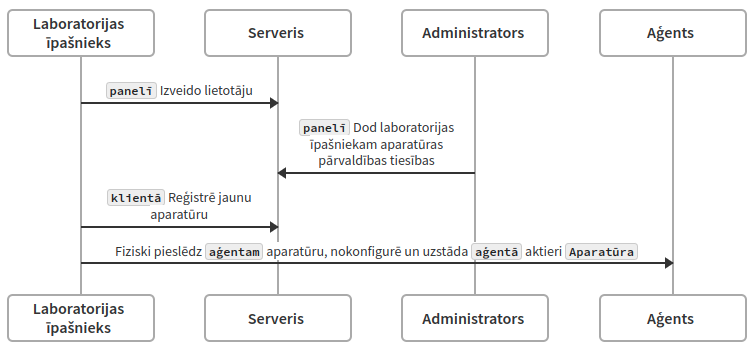
\includegraphics[width=1.0\linewidth]{assets/lab.png}
    \centering
    \caption{Platformas uzstādīšana laboratorijas digitalizācijai.}
    \label{fig:labsetup}
\end{figure}

Lai sajustu, kāda ir lietotāja pieredze, ir vērts novērtēt aģenta uzstādīšanas
komandu \ref{lst:agentconfig}, kas izveido \glslink{actor}{aktieri}
\lstinline!Aparatura!, izveido savienojumu ar \glslink{server}{serveri} un veic
\glslink{board}{aparatūras} pārvaldību pēc \glslink{server}{servera} komandām.
Minētā komanda informē komandu rindas rīku, ka \glslink{board}{aparatūra} ir
Digilent Anvyl paveida \lstinline!agent-anvyl!, platformā
\glslink{board}{aparatūra} ir reģistrēta ar noteiktu identifikatoru
\lstinline!-b ...!, fiziski piesaistītā \glslink{board}{aparatūra} ir ar
noteiktiem konfigurēšanas/programmēšanas parametriem \lstinline!-n ... -s ...!
un ka \glslink{board}{aparatūrai} ir pieejams noteikts seriālās komunikācijas
ports \lstinline!-f ...!.

\begin{lstlisting}[caption={\gls{dip} aģenta uzstādīšana komandu rindā},label={lst:agentconfig},captionpos=b]
dip_client agent-anvyl -b 5b17a393-9004-40ec-a9db-e0bb1e77a0e6 -n Anvyl \
    -s 0 -f /dev/serial/by-id/usb-Digilent_...-if01-port0
\end{lstlisting}

Attēlā \ref{fig:development} aprakstīts kā izskatītos izstrādātāja platformas
izmantošana, lai digitāli un attālināti bez tiešas, fiziskas
\glslink{board}{aparatūras} piekļuves veiktu \glslink{board}{aparatūras}
programmēšanu, testēšanu un izmantošanu. Kā arī komandā \ref{lst:quickrun} ir
redzams, ka, lai gan programmēšanas mehānisms pamatā ir sarežģīts, no
izstrādātāja skatpunkta \glslink{board}{aparatūras} attālināta programmēšana un
seriālā komunikācija var tikt abstrahēta gana, lai tas šķistu diezgan intuitīvi.
Komandā redzams norādījums izpildīt programmatūras augšupielādi
\glslink{server}{serverī} un \glslink{board}{aparatūrā}, un uzsākt seriālo
komunikāciju \lstinline!quick-run!, \glslink{board}{aparatūras} identifikators
platformā \lstinline!-b ...!, sakompilētas
\glslink{firmware}{programmaparatūras} faila ceļš izstrādātāja datorā
\lstinline!-f ...! un vēlamās izmantojamās \glslink{vinterface}{virtuālās
saskarnes} veids \lstinline!-t ...!.

\begin{lstlisting}[caption={\glslink{firmware}{Programmaparatūras} augšupielāde un seriālās komunikācijas komanda \gls{dip} klientā},label={lst:quickrun},captionpos=b]
dip_client quick-run -b f65e4276-2d72-4471-b5de-bddbc833d2ea \ 
    -f ./main.bit -t minos
\end{lstlisting}

\begin{figure}[H]
    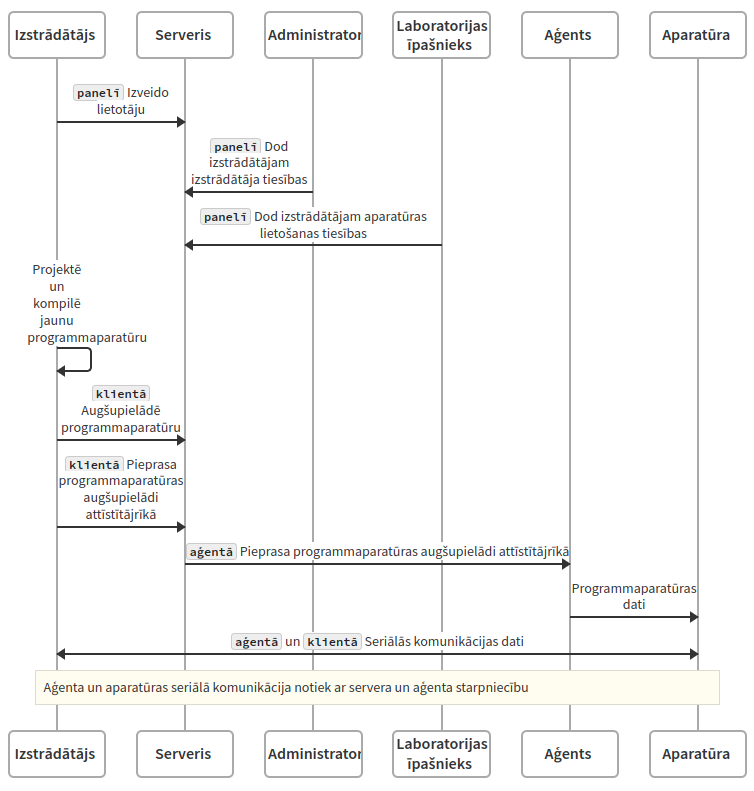
\includegraphics[width=1.0\linewidth]{assets/agent.png}
    \centering
    \caption{Attīstītājrīka aparatūras attālināta programmēšana.}
    \label{fig:development}
\end{figure}

\section{Tīmekļa kameras virtuālā saskarne}
\label{sec:vinweb}

Pēc darba vadītāja ieteikumiem, tika secināts, ka gadījumos, kad attālināta
\glslink{board}{aparatūras} programmēšana nefunkcionē korekti, būtu diezgan
grūti bez fiziskas klātbūtnes secināt, kas ir pie vainas, tādēļ būtu noderīgi,
ja būtu pieejama \glslink{board}{aparatūras} video straumēšana ar tīmekļa
kameru.

Lai realizētu šo funkcionalitāti, tika izveidoti dažādi \ref{sec:dipactorsystem}
nodaļā minēti \glslink{server}{servera} un aģenta \glslink{actor}{aktieri}, lai
veiktu tīmekļakameras datu starpniecību. Zemāk aprakstīts šo
\glslink{actor}{aktieru} dzīvescikls un ziņapmaiņa.

\begin{enumerate}
    \item Tīmekļa kameras datu avots ir ar komandu rindas rīku nokonfigurējams
        aktieris \lstinline!agent-video!
    \item \lstinline!agent-video! pievienojas \glslink{server}{serverim},
        tādējādi \glslink{server}{serverī} izveidojot aktieri
        \lstinline!server-video-control!, kas sūta atpakaļ
        \lstinline!agent-video! informāciju par straumes abonentu skaitu
    \item \lstinline!agent-video! no fiziski pievienotas tīmekļa kameras saņem
        video straumes datus
    \item Atkarībā no tā vai ir aktuāli video straumes abonenti,
        \lstinline!agent-video! sūta \lstinline!server-video-control! video
        straumes datus, lai ietaupītu patērētos tīkla resursus
    \item \glslink{server}{Serverī} \lstinline!server-video-control! publicē
        video straumes datus, izmantojot aktieri \lstinline!pub-sub!
    \item \glslink{mgmtpanel}{Pārvaldības panelim} pieslēdzas lietotāji,
        pieprasot video straumi, kas rezultē jauna aktiera izveidē
        \lstinline!server-video-subscriber!, kurš informē
        \lstinline!server-video-control! un \lstinline!pub-sub! par savu
        abonamentu
    \item \lstinline!pub-sub! saņemot video straumes datus no
        \lstinline!server-video-control!, pārtranslē šos datus arī
        \lstinline!server-video-subscriber!
    \item \lstinline!server-video-subscriber! aizsūta lietotājam atpakaļ HTTP
        \lstinline!application/ogg! atbildē aktuālos video straumes datus
\end{enumerate}

\begin{figure}[H]
    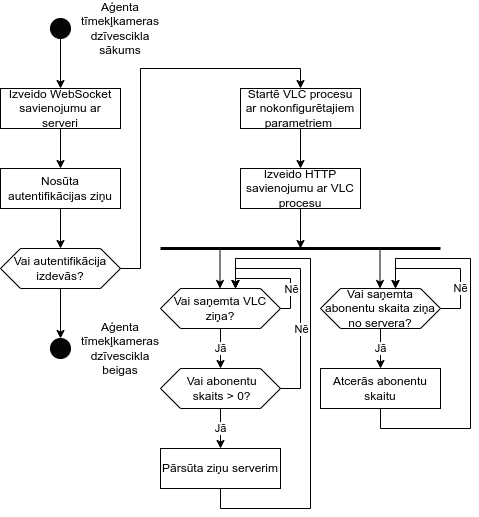
\includegraphics[width=0.6\linewidth]{assets/video_engine.drawio.png}
    \centering
    \caption{Tīmekļa kameras aģenta loģika.}
    \label{fig:videoengine}
\end{figure}

Attēlā \ref{fig:videoengine} ir redzama iepriekšminētā \lstinline!agent-video!
komandu rindas \glslink{actor}{aktiera} dzīvescikla loģika. Jāmin, ka brīžos,
kad jebkas noiet greizi, \glslink{actor}{aktieris} vienkārši izbeidz visus
aktīvos savienojumus un beidz darbu.

Savukārt, attēlos \ref{fig:mgmtpanelhw} un \ref{fig:hwstream} ir redzams
pārvaldības paneļa \glslink{board}{aparatūras} pārvaldības skats, no kura
iespējams sākt skatīties \glslink{board}{aparatūras} video straumi, kā arī
piemērs kā izskatās šāda video straume pārlūkā, precīzāk, kā izskatās publiski
pieejamā \cite{VeinbahsKrisjanisProduction} testa vides laboratorijas video
straume, kas tiek raidīta no darba autora mājām, Kalnciema ielā.

\begin{figure}[H]
    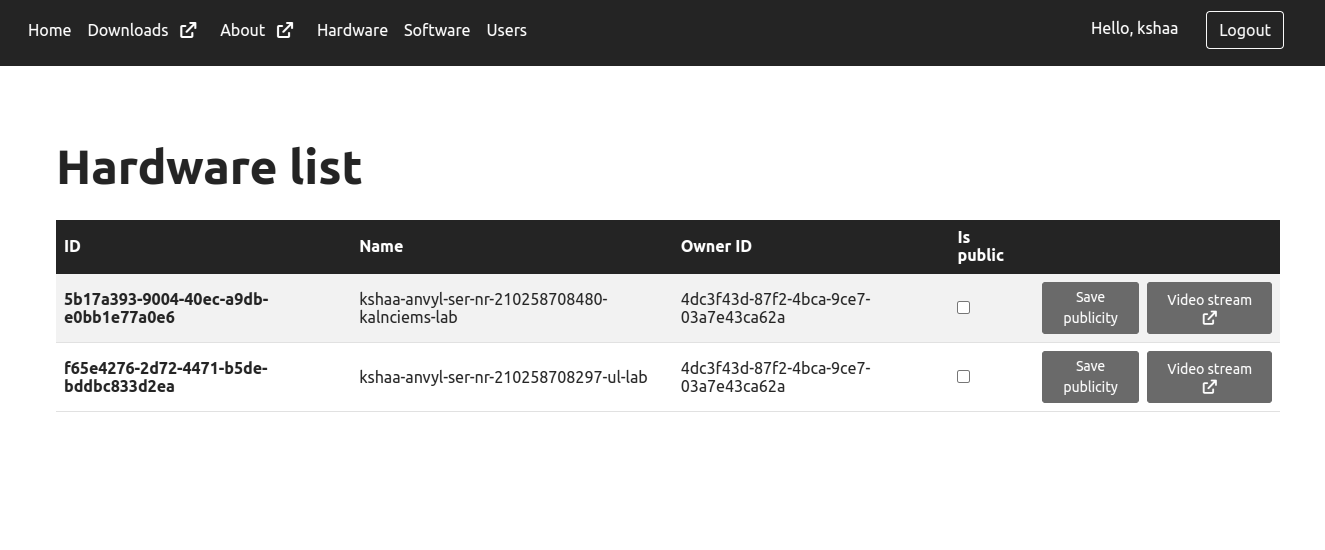
\includegraphics[width=0.9\linewidth]{assets/mgmt-panel-hw-gray.png}
    \centering
    \caption{Platformas pārvaldības paneļa lietotāju pārvaldības skats.}
    \label{fig:mgmtpanelhw}
\end{figure}

\begin{figure}[H]
    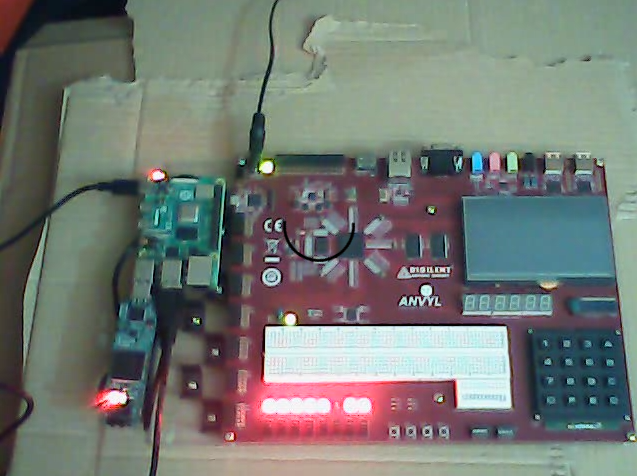
\includegraphics[width=0.9\linewidth]{assets/webcam-usage.png}
    \centering
    \caption{Pārvaldības paneļa aparatūras video straume.}
    \label{fig:hwstream}
\end{figure}

Diemžēl, jāmin, ka augstāk aprakstītajai video straumes translēšanas pieejai ir
pāris tehniskas un veiktspējas problēmas, kas tika atklātas izstrādes un
pētniecības laikā.

Pirmkārt, aģents ir izstrādāts Python programmēšanas valodā, kas nav īsti
paredzēta tādai paralēlai datu apstrādei, kas realizēta tīmekļa kameras datu
straumēšanas \glslink{actor}{aktierī}.

Otrkārt, pārtranslēt VLC HTTP OGG straumi varētu nebūt pārāk efektīvi, labāk
būtu izmantot kādu bibliotēku, kas piedāvā šādu funkcionalitāti bez papildus
HTTP savienojuma nepieciešamības.

Treškārt, aģents ir mikrokontrolieris ar vājiem skaitļošanas resursiem, tādēļ
nav ieteicams, nedz pat īsti iespējams, no aģenta raidīt vairāk kā vienu
straumi, kas nozīmē, ka \glslink{server}{servera} pusē to ir jāduplicē ar
\gls{pubsub} mehānismiem, taču tas nebūt nav triviāli, jo video straumes datos
ir iekodēta dienasta informācija par to, kurš aktuālais kadrs šobrīd tiek
rādīts, kas, savukārt, ietekmē to kā \glslink{server}{serverim} ir jāizsūta HTTP
OGG atbildes, kas nozīmē, ka ir jāveic programmatiska video datu lasīšana vai
iespējams pat pārrakstīšana. Precīzāk, sūtot HTTP \lstinline!application/ogg!
atbildes daļas, ir nepieciešams norādīt \lstinline!Range! galveni, kas saturētu
informāciju par to kurā video straumes laikā parādās minētie video dati.
\cite[para. 14.35.2]{RFC2616} Šī informācija ir iekodēta OGG lapās laukā
\lstinline!granule_position! \cite[para 6., A]{RFC3533}, taču, lai to nolasītu
ir jāizstrādā OGG lapu parseris, ko darba izstrādes laika ierobežojumu dēļ
nebija iespējams laicīgi izdarīt. Darba ietvaros šim trešajam punktam tika
realizēti dažādi aprisinājumi (1. straumes sākšana no jauna katru reizi, kad ir
jauns abonents, 2. straumes pirmo lapu atcerēšanās un sākotnēja nosūtēšana
tādējādi imitējot straumes korektu sākumu, kam seko pārrāvums līdz aktuālajam
brīdim), taču tie nebija pārāk augstas kvalitātes, kas rezultēja straumes lēnumā
un pārrāvumos. 

\section{Baitu virtuālās saskarnes}
\label{sec:vinbytes}

Pats primitīvākais veids kā uzturēt seriālo komunikāciju ir sūtīt uz un no
\glslink{board}{aparatūras} baitus. Izmantojot šādu primitīvu komunikācijas
mehānismu, lai lietotājs varētu attālināti mijiedarboties ar
\glslink{board}{aparatūru}, ir izstrādātas divas virtuālas
\glslink{vinterface}{saskarnes}, kas realizētas 1) kā termināļa tekstuāla
saskarne un 2) kā termināļa grafiskā saskarne.

Tekstuālā baitu līmeņa termināļa saskarne komandu rindas rīkā tiek dēvēta par
\lstinline!hexbytes!, izmantojot šo tekstuālo saskarni
\glslink{board}{aparatūras} lietotājam jeb, ticamāk, izstrādātājam ir iespējams
nolasīt no \glslink{board}{aparatūras} nākošos baitus kā heksidecimālu simbolu
virkni, savukārt, \glslink{board}{aparatūrā} ir iespējams sūtīt baitus spiežot
datora klaviatūras spiedpogas, kas tiek interpretētas kā ASCII simboli, kuru
baitu vērtība tiek sūtīta uz \glslink{board}{aparatūru}. Šādas tekstuālas
virtuālās \glslink{vinterface}{saskarnes} pielietojumu, izmantojot platformas
komandu rindas rīku, var skatīt tekstā \ref{lst:hexbytes}, kur redzama
attālināta pieslēgšanās noteiktas \glslink{board}{aparatūras} (pēc platformā
reģistrēta identifikatora) seriālajam portam, izmantojot virtuālo
\glslink{vinterface}{saskarni} \ref{lst:hexbytes}, kas tiek pārtraukta procesam
nododot \lstinline!SIGINT! signālu, izmantojot \lstinline!Ctrl+C! klaviatūras
spiedpogu kombināciju.

\begin{lstlisting}[caption={\lstinline!hexbytes! izmantošana no komandu rindas},label={lst:hexbytes},captionpos=b]
$ dip_client hardware-serial-monitor \
    -b f65e4276-2d72-4471-b5de-bddbc833d2ea -t hexbytes
[0x0] [0x2] [0x2e] [0x0] [0x1] [0x0] [0x6] 
[0x0] [0x0] [0x0] [0x0] [0x0] [0x1] [0x0] [0x6]  
Success: Finished monitoring
\end{lstlisting}

Grafiskā baitu līmeņa termināļa saskarne komandu rindas rīkā tiek dēvēta par
\lstinline!buttonleds!, programmatiski tā funkcionē tāpat kā iepriekšminētā
virtuālā \glslink{vinterface}{saskarne}, jo baiti tiek sūtīti uz
\glslink{board}{aparatūru} un baiti tiek saņemti no \glslink{board}{aparatūras},
taču lietotājam šī mijiedarbība tiek pasniegta izmantojot grafisku saskarni,
kurā ir 24 spiedpogas baitu vērtībā no \lstinline!0x00! līdz \lstinline!0x17! un
8 LED gaismas 8 bitu jeb baita vērtībā. Šīs virtuālās
\glslink{vinterface}{saskarnes} izsaukums redzams tekstā \ref{lst:buttonleds} un
saskarnes izskats attēlā \ref{fig:buttonleds}.

\begin{lstlisting}[caption={\lstinline!buttonleds! izsaukums no komandu rindas},label={lst:buttonleds},captionpos=b]
$ dip_client hardware-serial-monitor \
    -b f65e4276-2d72-4471-b5de-bddbc833d2ea -t buttonleds
[2022-04-29 21:37:24] [INFO] [monitor_button_led_bytes_app] Starting app
[2022-04-29 21:37:50] [INFO] [monitor_button_led_bytes_app] App finished
Success: Finished monitoring
\end{lstlisting}

\begin{figure}[H]
    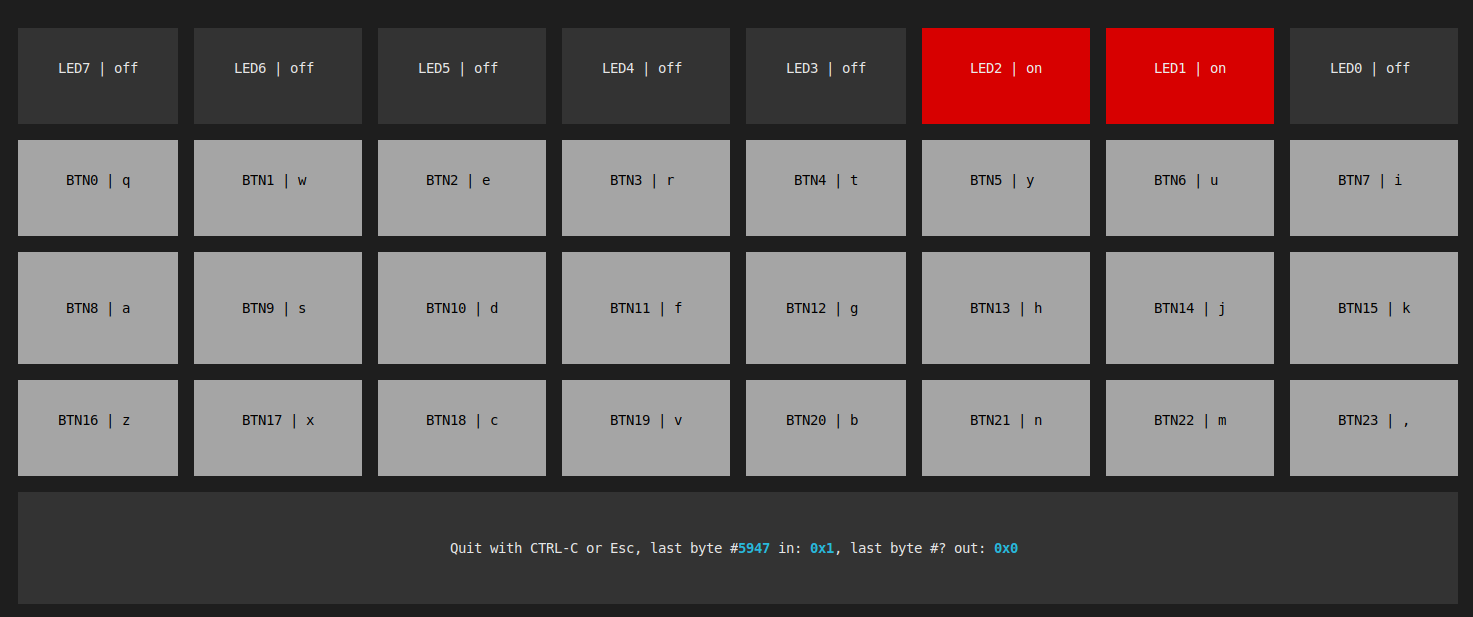
\includegraphics[width=0.9\linewidth]{assets/buttonleds.png}
    \centering
    \caption{\lstinline!buttonleds! virtuālā grafiskā saskarne}
    \label{fig:buttonleds}
\end{figure}

Šādas baitu līmeņa \glslink{vinterface}{saskarnes} jau ir ļoti spējīgas, ar tām var piemēram,
projektēt galīgu stāvokļu automātus vai pat šādus automātus, kas veic darbības
ar papildus reģistru atmiņu. Un spiedpogas var izmantot kā ievaddatus, lai
darbinātu šādu automātu stāvokļu pārejas.

Tomēr šādām \glslink{vinterface}{saskarnēm} ir trūkums - vienā sūtījumā ir
pieejams tikai viens baits, kas patiesībā nav daudz, it īpaši, ja sūtījumā vēlas
sūtīt dažāda veida datus. Ja nu ir nepieciešamība sūtīt 4 slēdžu aktuālos datus
un spiedpogu ievaddatus? Tad izsūtītajā baitā 4 biti jāizmanto slēdžu vērtībām
un pārējie 4 spiedpogu vērtībām. Bet ko darīt, ja jāizsūta 16 slēdžu vērtības?
Tad ar baitu vairs nepietiek, nepieciešami vairāki baiti, tādēļ tika izstrādāta
sarežģītāka virtuālā saskarne "MinOS" (no angl. minimal operating system), kas
aprakstīta nodaļā \ref{sec:vinminos}.

\section{Multifunkcionāla virtuālā saskarne "MinOS"}
\label{sec:vinminos}

Multifunkcionālā virtuālā \glslink{vinterface}{saskarne} "MinOS" (no angl.
minimal operating system), kas sastāv no vairākiem grafiskiem elementiem, ir
virtuāla \glslink{vinterface}{saskarne}, lai vairākos veidos vienā
\glslink{vinterface}{saskarnē} mijiedarbotos ar attīstītājrīku aparatūru, kas ir
realizēta kā termināļa grafiskā saskarne, kas redzama attēlā \ref{fig:minosgui}
un konceptuāli tā līdzinās tai pašai fiziskai saskarnei, kas pieejama uz Anvyl
attīstītājrīka, kas redzama attēlā \ref{fig:anvyl}. 

Skatoties attēla \ref{fig:minosgui} \glslink{vinterface}{saskarnē}, ir redzams
8x8 RGB displejs (skat. kreiso daļu), 8 sarkanas LED gaismas (skat. labās puses
1. rindu), 8 sarkani LED slēdži (skat. labās puses 2. rindu), 3x8 pelēkas
spiedpogas (skat. labās puses 3.-5. rindu), teksta lauki (skat. labās puses
6.-7. rindu). 

\begin{figure}[H]
    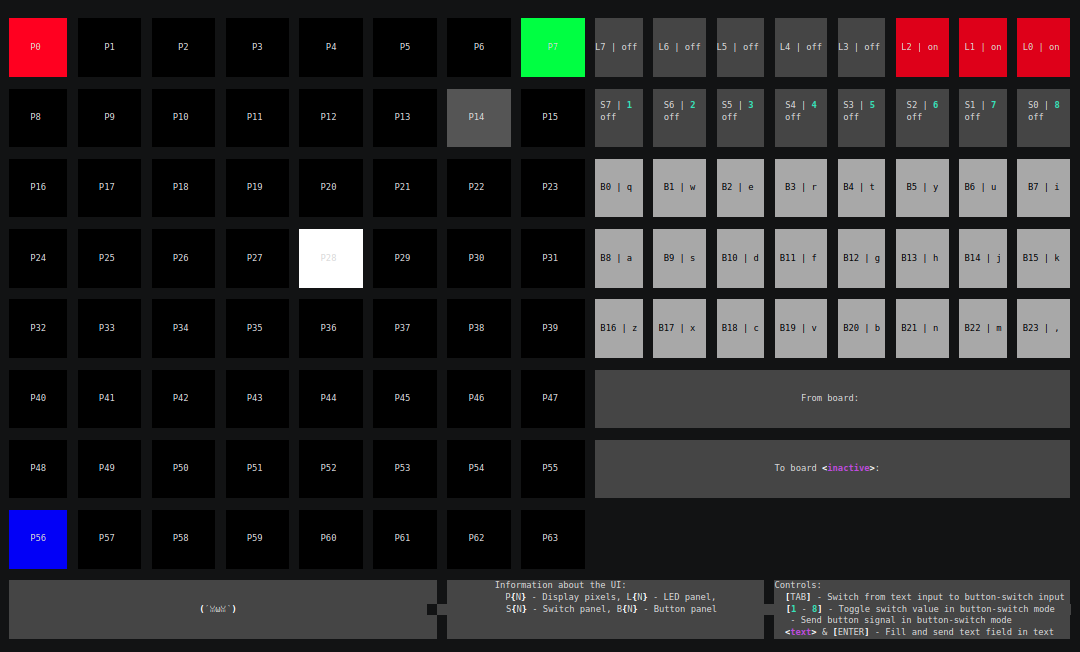
\includegraphics[width=1.0\linewidth]{assets/min-os-execution.png}
    \centering
    \caption{MinOS termināļa grafiskā saskarne.}
    \label{fig:minosgui}
\end{figure}

\begin{figure}[H]
    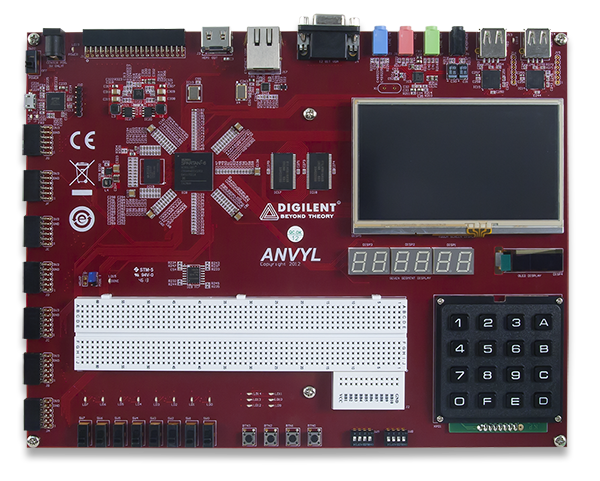
\includegraphics[width=0.7\linewidth]{assets/anvyl.png}
    \centering
    \caption{Anvyl attīstītājrīks.}
    \label{fig:anvyl}
\end{figure}

Lai realizētu MinOS virtuālo \glslink{vinterface}{saskarni} ir nepieciešams uz
un no aparatūras sūtīt dažāda veida datus. Gana daudz, lai ar vienu baitu
nepietiktu, jo lai izsūtītu 64 pikseļu RGB displejam pat viena pikseļa datus ir
nepieciešami 6 biti krāsai (\(2^2 * 3\)) un vēl 6 biti indeksam
(\(\log_{2}64\)), tātad kopā 12 biti, kas ir vairāk par 8 bitiem jeb baitu, kas
izmantots iepriekšminētās virtuālās \glslink{vinterface}{saskarnēs}. Un MinOS
\glslink{vinterface}{saskarnē} vēlamo elementu ir vairāk nekā tikai RGB
displejs, tādēļ nepieciešams protokols, lai sūtītu vairāku veidu baitu ziņas
seriālajā komunikācijā.

MinOS \glslink{vinterface}{saskarnes} vairāku baitu ziņapmaiņai tika izplānots
komunikācijas protokols starp \glslink{board}{aparatūru} un klientu. Protokols
tika formāli definēts, izstrādājot BNF formāta sintaksi, kuru iespējams apskatīt
pielikumā \ref{att:minosbnf}. Ņemot vērā, ka vēlamais protokols ir binārs, tad
BNF formāts definē baitus kā heksidecimālu ciparu pārus tātad formātā
\lstinline!0x??!.

Kā piemērs ziņai, kas atbilst pielikumā pieejamajam BNF formātam ir binārā ziņa
\ref{lst:minosledchunk}, kas MinOS \glslink{vinterface}{saskarnē} tiek
izmantota, lai sūtītu LED gaismas datus no \glslink{board}{aparatūras} uz
klientu grafiskai attēlošanai.

\begin{lstlisting}[caption={MinOS LED gaismu pakete},label={lst:minosledchunk},captionpos=b]
    0x00 0x02 0xFF 0x00 0x01 
\end{lstlisting}

MinOS ziņapmaiņas protokols rakstiskā valodā ir sekojošs.
\begin{enumerate}
    \item Baitu straumē var sastapt diva veida simbolus:
    \begin{enumerate}
        \item \lstinline!escaped! simbolus
        \item ne \lstinline!escaped! simbolus
    \end{enumerate}
    \item \lstinline!escaped! simboli ir jebkurš baits, pirms kura iepriekšējais ir baits ir \lstinline!0x00!
    \item Ne \lstinline!escaped! simbols ir tāds, pirms kura iepriekšējais baits nav \lstinline!0x00!
    \item Ja baitu straumē sastopams \lstinline!0x00 0x00!, tad jāpieņem, ka
        sākotnējā \lstinline!escaped! simbola sūtīšana netika korekti pabeigta
        un ir sākusies nākamā \lstinline!escaped! simbola sūtīšana
    \item Ir diva veida \lstinline!escaped! simboli: 
    \begin{enumerate}
        \item Ziņas beigu simbols \lstinline!0x01!
        \item Tipizētas ziņas sākuma simbols \(x\), kur \(x\geq0x02\)
    \end{enumerate}
\end{enumerate}

Ar šādu protokola definīciju ir iespējams sūtīt vairāku baitu ziņas, kur katrai
ziņai piemīt tips, kas ir skaitlis vērtībā no \(0\) līdz \(2^8-2\). Šis
protokols arī ir izmantots MinOS \glslink{vinterface}{saskarnē}, lai sūtītu
ziņas no lietotāja \glslink{board}{aparatūrai} un otrādi. 

Kā piemēru skatoties iepriekšminēto LED gaismas ziņu \ref{lst:minosledchunk}
varam redzēt, ka ziņa sākas ar \lstinline!0x00 0x02!, tātad LED gaismas ziņas
tips ir \(0x02 - 2 = 0x00\) jeb \(0\), redzams, ka ziņa korekti beidzas ar
simbolu \lstinline!0x00 0x01!. Un ziņai pa vidu ir vērtība \lstinline!0xFF!, kas
apzīmē, ka no 8 LED gaismām visas ir ieslēgtas (visi 8 biti ir ar vērtību 1). Ja
šo ziņu pārbauda ar kādu tiešsaistē pieejamu BNF sintakses pārbaudes rīku,
piemēram, BNF playground, \cite{BNFPlayground} pret simbolu \lstinline!<chunk>!,
izmantojot pielikumā definēto protokola sintaksi, kas ir ziņas simbols, tad šī
ziņa veiksmīgi iziet pārbaudi.

Daļa no šāda protokola izstrādes sarežģītības nāk ne tikai no tā plānošanas, bet
arī no tā realizācijas, jo jāatcerās, ka, lai gan realizēt parseri Python
programmēšanas valodā ir triviāli, realizēt to Verilog
\glslink{firmware}{programmaparatūrā} ir grūtāk.

Attēlā \ref{fig:chunkparser} redzams galīgs determinēts stāvokļu automāts, kas
realizē pielikumā pieejamās BNF sintakses parsēšanu, nolasot ziņas tipu un
datus. Gadījumos, kad ievaddati neatbilst nevienai pārejai, automāts paliek tajā
pašā stāvoklī, kurā jau šobrīd atrodās. Attēlā redzamās pārejas pirmajā rindā
satur pārejas ievaddatu nosacījumus un otrā rindā, pārejas blakusefektus jeb
izpildītās darbības. Šis automāts nav pilnīgs, jo patiesībā ir nepieciešami
papildus dienasta dati, lai glabātu aktuālo parsētās ziņas indeksu datu buferī,
taču šī loģika netika ielikta ilustrācijā, lai to pārāk nesarežģītu. Šādu
automātu ir iespējams vienkārši realizēt gan Verilog valodā, gan Python valodā,
kas arī tika darīts, lai realizētu MinOS virtuālo saskarni.

Automātā pieminētie ievaddati ir ielasītā baita gatavība
\lstinline!is_rx_ready!, ielasītā baita vērtība \lstinline!rx_data!. Automātā
pieminētie izvaddati ir ziņas veids \lstinline!r_chunk_type! un ziņas datu
buferis \lstinline!r_chunk_bytes!. Automātā pieminēta arī palīgvērtība - ziņas
aktuālā baita indekss buferī \lstinline!buffer_index!.

\begin{figure}[H]
    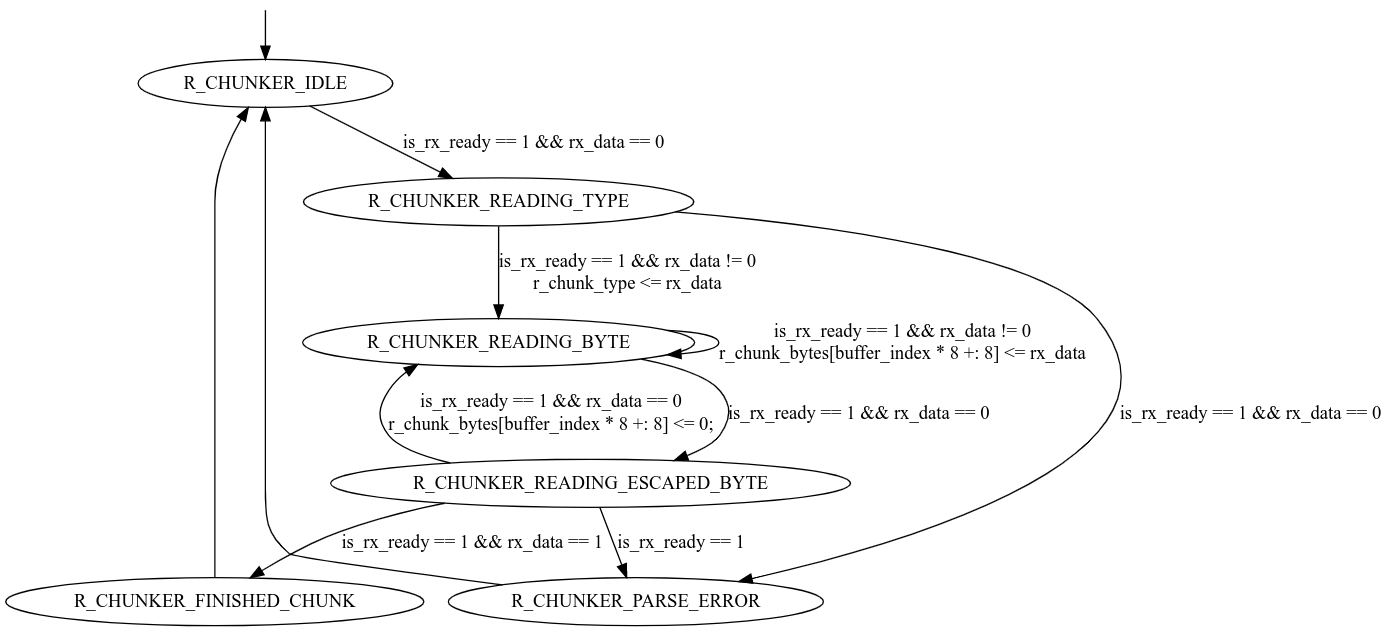
\includegraphics[width=1.0\linewidth]{assets/chunkparser.png}
    \centering
    \caption{MinOS ziņu parsera galīgs determinēts automāts.}
    \label{fig:chunkparser}
\end{figure}

Lai gan lejupielādējot platformas klienta komandu rindas rīku uzreiz ir pieejama
Python valodā programmētā grafiskā saskarne, tomēr attīstītājrīkā ir
nepieciešama atbilstoša \gls{firmware}, kas komunicē izmantojot MinOS protokolu,
tādēļ projekta ietvaros Verilog valodā tika izstrādāts MinOS modulis, kas
abstrahē seriālo komunikāciju un izstrādātājam izvērš tikai interesējošos
virtuālās \glslink{vinterface}{saskarnes} elementus. Attēlā \ref{fig:minos} redzama šī Verilog moduļa
grafiskā interpretācija. 

\begin{figure}[H]
    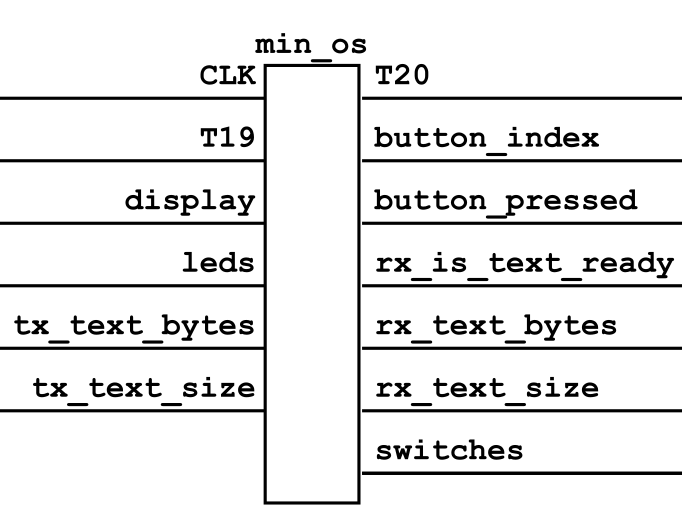
\includegraphics[width=0.7\linewidth]{assets/min-os-grey.png}
    \centering
    \caption{MinOS \glslink{firmware}{programmaparatūras} modulis.}
    \label{fig:minos}
\end{figure}

Attēlā \ref{fig:minos} redzamais Verilog valodā izstrādātais modulis izvērš
dažādus signālus, lai mijiedarbotos ar attālināto grafisko lietotāja MinOS
\glslink{vinterface}{saskarni}. Tabulā \ref{table:minossignals} ir dokumentēti
no moduļa izvērstie signāli un to būtība.

\begin{table}[H]
    \newcounter{minossignalcounter}
    \newcommand\rownumber{\stepcounter{minossignalcounter}\arabic{minossignalcounter}.}
    \begin{tabular}{ |p{1cm}|p{3cm}|p{2cm}|p{3cm}|p{6cm}| }
    \hline
    N.p.k.&Signāls&Virziens&Izmērs&Būtība \\
    \hline
    \rownumber&\lstinline!CLK!&I&1&Pulksteņa signāls \\
    \hline
    \rownumber&\lstinline!T19!&I&1&Seriālā porta ievaddatu signāls \\
    \hline
    \rownumber&\lstinline!display!&I&\(64 * 8 = 512\)&Displeja pikseļu krāsas datu signāls \\
    \hline
    \rownumber&\lstinline!leds!&I&8&LED gaismu signāli \\
    \hline
    \rownumber&\lstinline!tx_text_bytes!&I&\(32 * 8 = 256\)&Izsūtītā ASCII teksta datu signāls \\
    \hline
    \rownumber&\lstinline!tx_text_size!&I&8&Izsūtītā ASCII teksta izmēra signāls \\
    \hline
    \rownumber&\lstinline!T20!&O&1&Seriālā porta izvaddatu signāls \\
    \hline
    \rownumber&\lstinline!button_index!&O&1&Nospiestās spiedpogas indeksa signāls \\
    \hline
    \rownumber&\lstinline!button_pressed!&O&1&Spiedpogas nospiešanas stāvokļa signāls \\
    \hline
    \rownumber&\lstinline!rx_is_text_ready!&O&1&Iesūtītā ASCII teksta gatavības signāls \\
    \hline
    \rownumber&\lstinline!rx_text_bytes!&O&\(32 * 8 = 256\)&Iesūtītā ASCII teksta datu signāls \\
    \hline
    \rownumber&\lstinline!rx_text_size!&O&8&Iesūtītā ASCII teksta izmēra signāls \\
    \hline
    \rownumber&\lstinline!switches!&O&8&Slēdžu stāvokļu signāls \\
    \hline
    \end{tabular}
    \centering
    \captionsetup{justification=centering}
    \caption{Verilog MinOS moduļa signāli, I - ievad signāls, O - izvadsignāls}
    \label{table:minossignals}
\end{table}

Ar šādu virtuālu \glslink{vinterface}{saskarni} un tās Verilog realizāciju jau ir iespējams projektēt
daudz sarežģītākas digitālas iekārtas. Tehniski, ņemot vērā, ka ir pieejams 64
RGB krāsu monitors un spiedpogas, būtu jābūt iespējai ar šādu abstrakciju
attālināti projektēt, testēt un spēlēt datorspēli "Tetris" tikpat ārti kā esot
fiziski klāt attīstītājrīku \glslink{board}{aparatūrai}, kas ir cienījams
sasniegums!

Būtu vērtīgi līdz galam definēt ziņas, kādas atbalsta MinOS
\glslink{vinterface}{saskarne}. Kā jau iepriekš ilustrēts, MinOS
\glslink{vinterface}{saskarne} atbalsta sūtīt ziņu par LED gaismu stāvokli.
Visas MinOS atbalstītās ziņas, savukārt, aprakstītas tabulā
\ref{table:minospackets}.

\begin{table}[H]
    \newcounter{minospacketcounter}
    \newcommand\rownumber{\stepcounter{minospacketcounter}\arabic{minospacketcounter}.}
    \begin{tabular}{ |p{1cm}|p{3cm}|p{2cm}|p{8cm}| }
    \hline
    N.p.k.&Nosaukums&Izmērs&Būtība \\
    \hline
    \rownumber&\lstinline!leds!&1 baits&8 LED gaismu stāvoklis \\
    \hline
    \rownumber&\lstinline!switches!&1 baits&8 slēdžu stāvoklis \\
    \hline
    \rownumber&\lstinline!buttons!&1 baits&\(2^8\) spiedpogu nospiešanas fakts \\
    \hline
    \rownumber&\lstinline!display!&2 baiti&6 biti pikseļa indeksam, 6 biti pikseļa RGB krāsu vērtībām \\
    \hline
    \rownumber&\lstinline!text!&32 baiti&ASCII teksta vērtība \\
    \hline
    \end{tabular}
    \centering
    \captionsetup{justification=centering}
    \caption{MinOS virtuālās saskarnes atbalstītās ziņas}
    \label{table:minospackets}
\end{table}

Atsaucoties uz nodaļas sākumu, attēlā \ref{fig:minosgui}, ir ekrānuzņēmums no
MinOS virtuālās \glslink{vinterface}{saskarnes}, kuru darbina attēlā
\ref{fig:minosusage} redzamā demo jeb parauga \gls{firmware}, kas tika
izstrādāta, lai atrādītu MinOS darboties spēju.

\begin{figure}[H]
    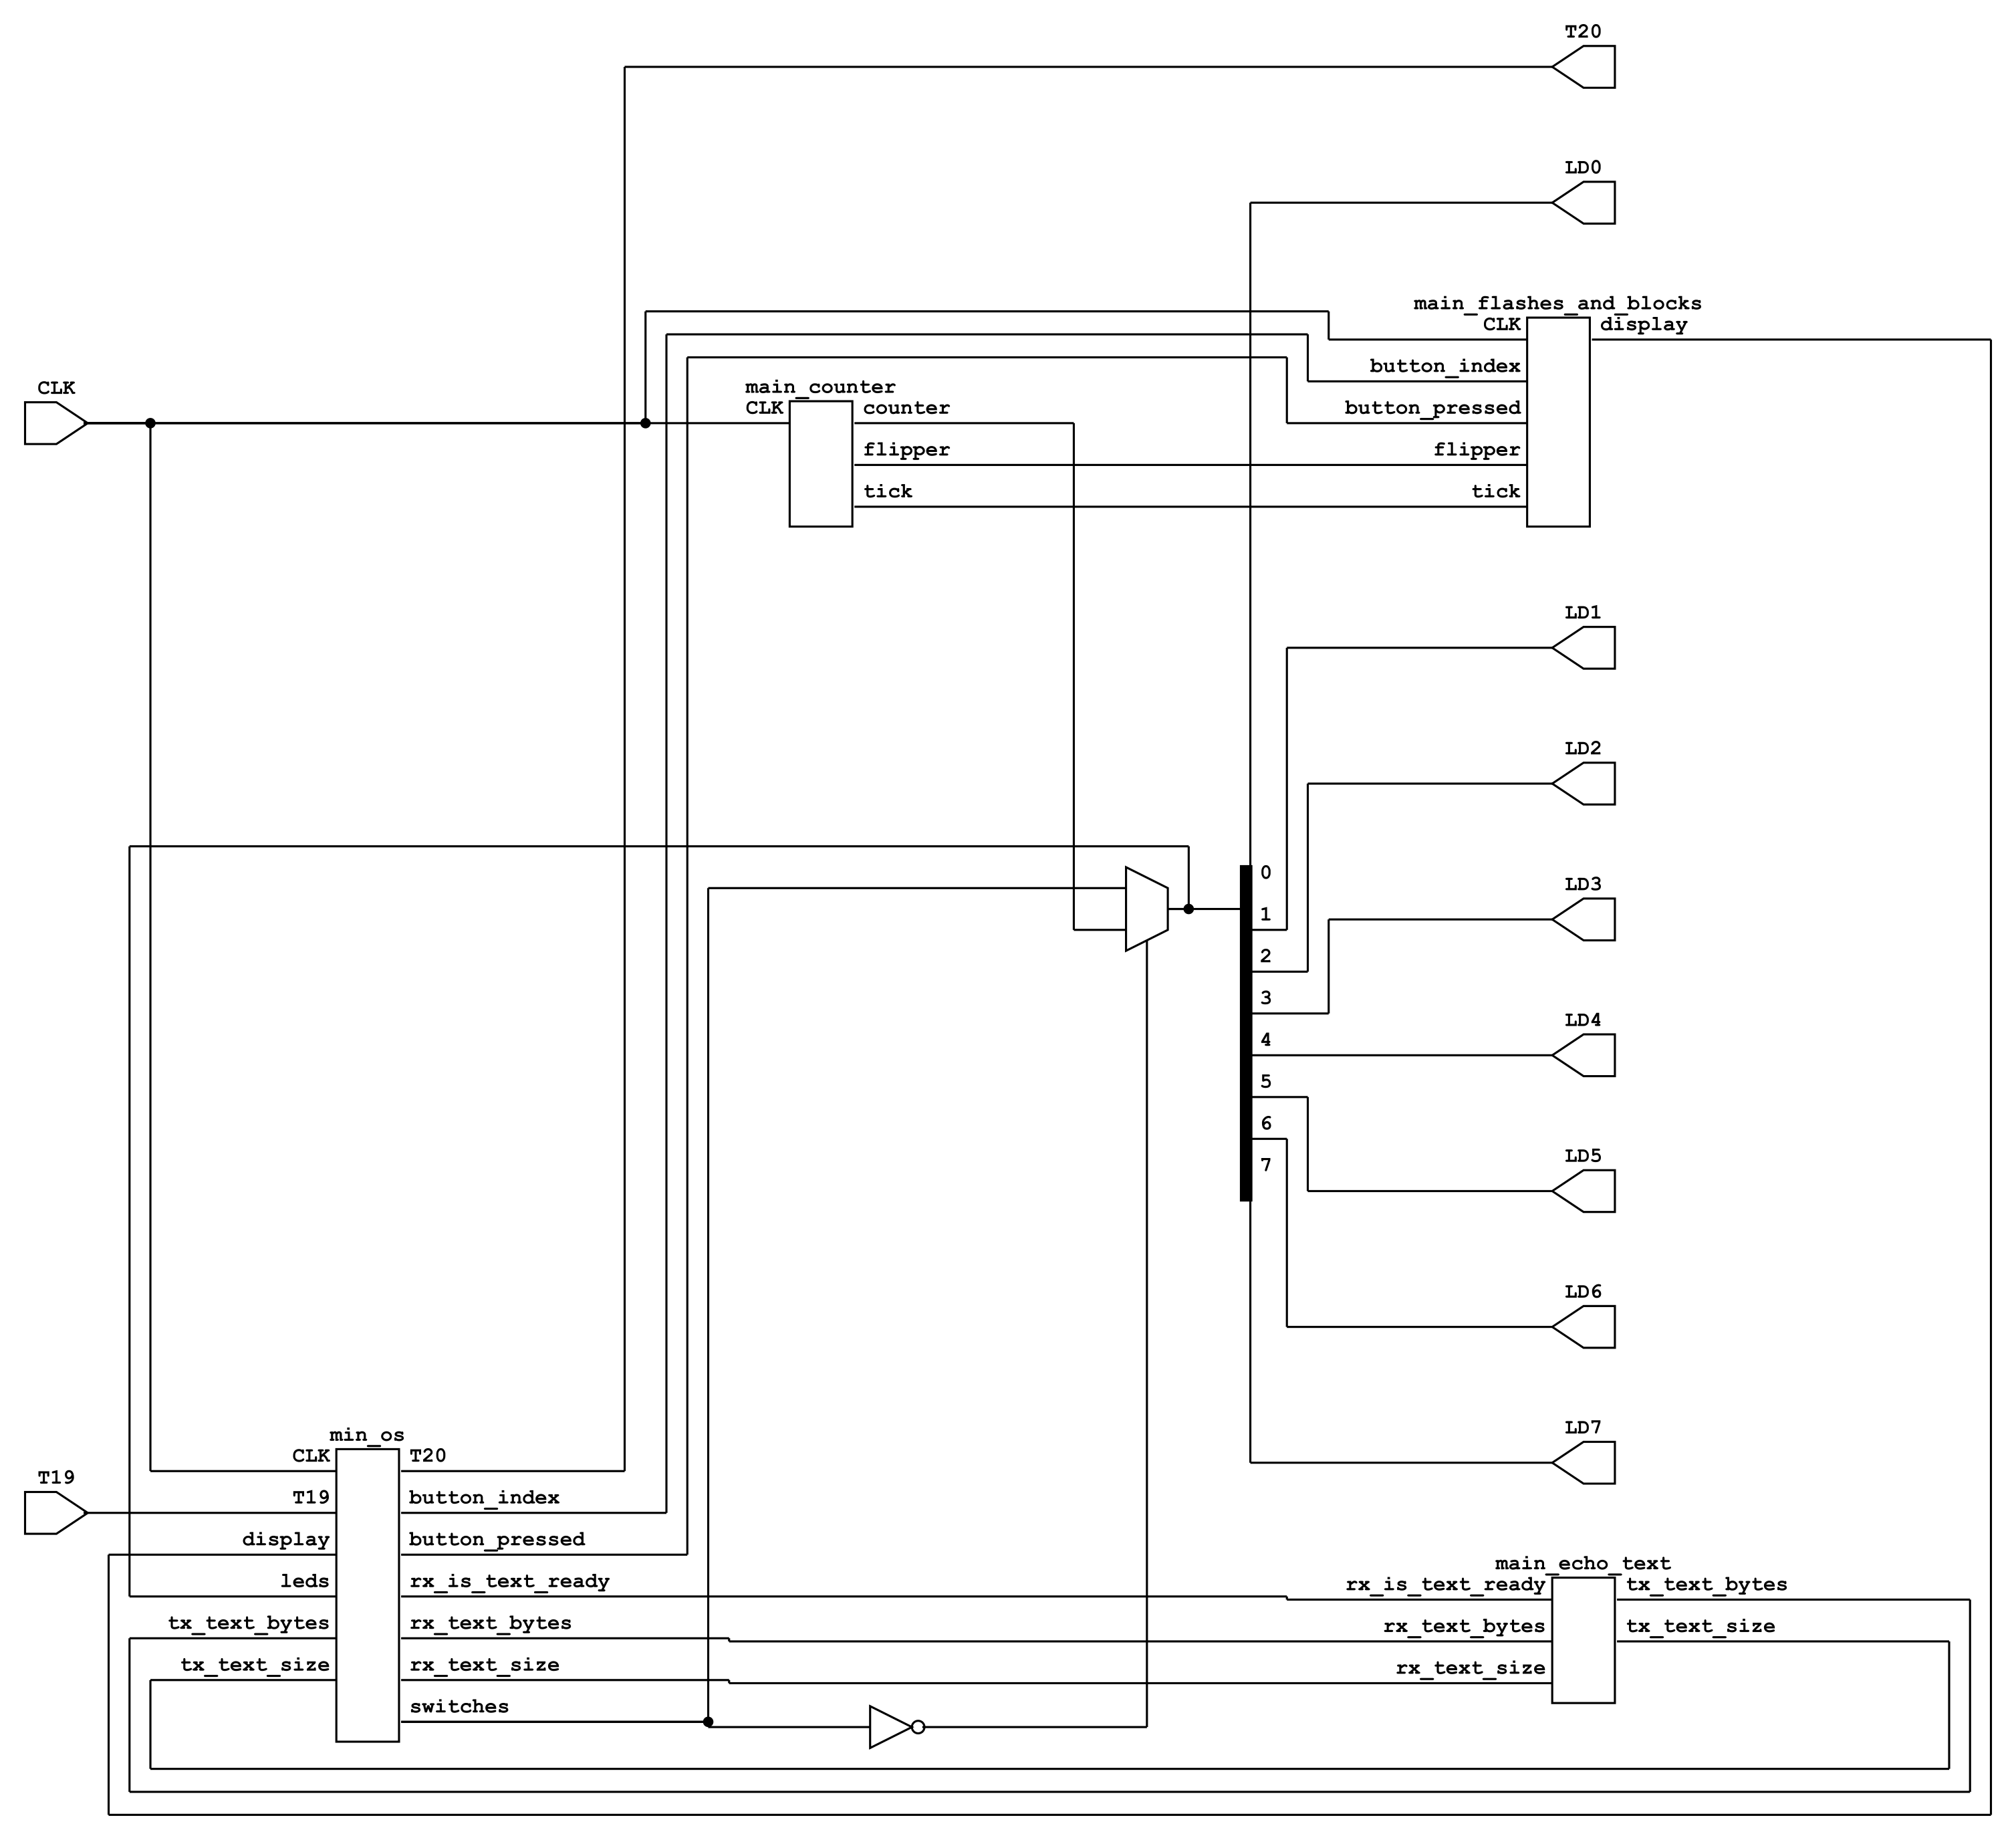
\includegraphics[width=1.0\linewidth]{assets/min-os-usage-grey.png}
    \centering
    \caption{MinOS \glslink{firmware}{programmaparatūras} piemērs.}
    \label{fig:minosusage}
\end{figure}

Attēlā \ref{fig:minosusage} redzamā \gls{firmware} sastāv no četrām savienotām
moduļu shēmām. 

Kreisajā apakšējā stūrī ir projektā izstrādātais MinOS protokola seriālās
komunikācijas abstrakcijas modulis \lstinline!min_os!, attēla sānos ir
\gls{fpga} porti \lstinline!CLK!, \lstinline!T19!, \lstinline!T20!,
\lstinline!LD0-7!, kas aprakstīti arī tabulā \ref{table:minossignals}, izņemot
\lstinline!LD0-7!, kas nav MinOS specifiski, bet ir vienkārši fiziskas gaismas
diodes, kas ir pieejamas uz Anvyl attīstītājrīka, ko izstrādātā demo
\gls{firmware} izmanto papildus. 

Papildus šiem tipiskajiem moduļiem ir trīs demo
\glslink{firmware}{programmaparatūrai} specifiski moduļi. Pirmkārt, pa vidu
augšā \lstinline!main_counter!, kas katru sekundi uz vienu tikšķi paceļ signālu
\lstinline!tick!, katru sekundi maina vērtību signālam \lstinline!flipper!,
katru sekundi pieskaita 8 bitu signālam \lstinline!counter! skaitli
\lstinline!0x01!. Otrkārt, pa labi apakšā modulis \lstinline!main_echo_text!
saņem no lietotāja saskarnes sūtītu tekstu un pārsūta to atpakaļ saskarnei.
Treškārt, pa labi augšā modulis \lstinline!main_flashes_and_blocks! reaģē uz
spiedpogu signāliem un funkcionē kā RGB displeja dzinis.

Rezultātē \gls{firmware} nodrošina sekojošu \glslink{vinterface}{saskarnes} demo funkcionalitāti.
\begin{enumerate}
    \item RGB monitorā katru sekundi trīs stūros mirkšķ sarkana, zaļa un zila
        gaisma
    \item Saskarnē izmantojot WASD un TFGH spiedpogas, monitorā ir kustināmi uz
        visām pusēm divi dažādu pelēku krāsu pikseļi
    \item Sarkanās LED gaismas skaita no \lstinline!0! līdz \lstinline!255!,
        ilustrējot šo skaitli gaismās kā 8 bitu vērtību
    \item Ja kāds no slēdžiem ir ieslēgts, tad LED gaismas spoguļo slēdžu
        vērtību
    \item Jebkurš teksts, kas tiek iesūtīts aparatūrai tiek atsūtīts atpakaļ
        identiski saskarnē
\end{enumerate}

Lai gan attēls \ref{fig:minosgui} ir statisks un nespēj šo funkcionalitāti
atrādīt, eksistē arī publiski internetā, YouTube platformā, pieejams video ar
šīs demo \glslink{firmware}{programmaparatūru} un MinOS
\glslink{vinterface}{saskarni}.
\cite{VeinbahsKrisjanisDemo} 

\section{Infrastruktūras pārvaldība}
\label{sec:ops}

Attēlā \ref{fig:hwstream} redzama demo laboratorija, kas uzstādīta darba autora
mājās, Kalnciema ielā. Lai gan nodaļā \ref{sec:dipplatform} redzamā 0. līmeņa
DPD diagramma, šķietami, gana ilustrē platformas konceptuālo uzbūvi, iespējams
ir vērtīgi aplūkot fiziskā līmenī izmantoto publisko testa platformu
\cite{VeinbahsKrisjanisProduction}. Attēlā \ref{fig:production} redzama šāda
testa platformas fiziskā līmeņa arhitektūra. Testa platformas serveris tika
uzstādīts DigitalOcean mākoņpakalpojumu devēja virtuālmašīnā, kas atrodas datu
centrā Frankfurtē jeb Vācijā. Savukārt, pati laboratorija ar platformas aģentu
un \glslink{board}{aparatūru} atradās Kalnciema ielā jeb Latvijā. Arī
\glslink{firmware}{programmaparatūras} izstrādātājs jeb darba autors, atradās
Latvijā kafejnīcā ar bezvada tīklu.

\begin{figure}[H]
    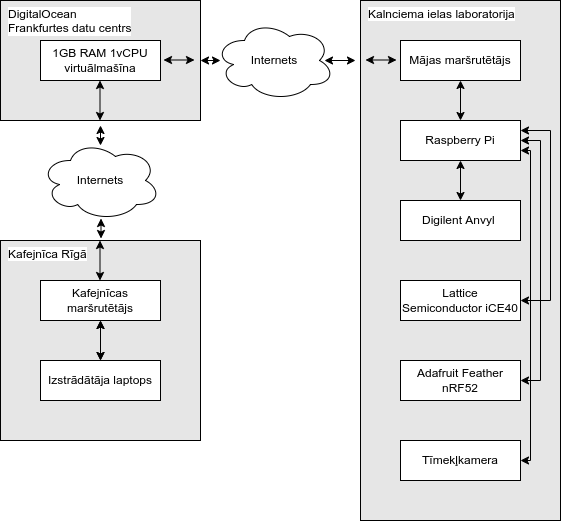
\includegraphics[width=0.8\linewidth]{assets/production.drawio.png}
    \centering
    \caption{Platformas testa vides fiziskā līmeņa arhitektūra.}
    \label{fig:production}
\end{figure}

Veicot attālinātu \glslink{firmware}{programmaparatūras} izstrādi datu plūsma
notika starp šo fizisko iekārtu tīklu. Tieši šajā arhitektūrā arī lielākoties
notika platformas izstrāde un testēšana tai skaitā demo
\glslink{firmware}{programmaparatūras} izstrāde un testēšana. Darba izstrādes
laikā tīkla latence starp šīm iekārtām nebija būtiski jūtama un būtiski
neietekmēja darba izstrādi.

Papildus jāmin, ka attēlā \ref{fig:production} redzama vairāk fiziska
\glslink{board}{aparatūra} nekā aprakstīta šajā darbā, taču oriģināli
prototipējot darba arhitektūru, tika secināts, ka arī šādas ierīces ir iespējams
pievienot platformai, taču laika ierobežojumu dēļ tām netika izstrādāts atbalsts
platformas komandu rindas aģenta rīkā. 


\chapter{Rezultāti}
\section{Laboratorijas uzstādīšana}

Īss apraksts kā uzstādīt laboratoriju jeb dzelžus platformā.

\section{Veļasmašīnas izstrāde platformā}

Īss apraksts kā projektēt veļasmašīnu un prototipēt to platformā.

\section{Datu apstrāde platformā}

Īss apraksts kā apstrādāt datus platformā.  

Ideja par to, ka var iesūtīt MinOS teksta paketi, saņemt atbildi JSON formātā.  

Jeb īsumā apraksts par to, ka var izmantot \gls{fpga} as a service iekš CLI.  

Ar domu: dipclient hardware-serial-monitor -t minosrequest -r "potat" -j true

\section{Veiktspēja}

Varētu aši uzcept kkādus benchmark ar to minosrequest un saprast, cik ātri var saņemt atbildes, cik ātri notiek apstrāde un tā.


%----------------------------------------------SECINĀJUMI----------------------------------------------------------

\chapter*{Secinājumi}
\addcontentsline{toc}{chapter}{Secinājumi}
Darba ietvaros ir izstrādāta digitālās \glslink{board}{aparatūras} projektēšanas
tiešsaistes platforma, kas iekļauj dažādus rīkus \glslink{board}{aparatūras}
izstrādātājiem un \glslink{board}{aparatūras} laboratoriju īpašniekiem.
\cite{VeinbahsKrisjanisTestbed}

Precīzāk, ir izstrādāta platforma, kas sastāv no klienta komandu rindas rīka
izstrādātājiem, lai augšupielādētu un testētu platformā
\glslink{firmware}{programmaparatūru}, aģenta komandu rindas rīka laboratorijas
īpašniekiem, lai attālināti pieslēgtu fizisku attīstītājrīku
\glslink{board}{aparatūru} platformai attālinātai programmēšanai un lietošanai.

Papildus platformas ietvaros izstrādāts \glslink{server}{serveris}, kurā
pārvaldīt dažādus lietotāju, \glslink{board}{aparatūras} un
\glslink{firmware}{programmaparatūras} datus un kas funkcionē kā vājas reāllaika
komunikācijas starpnieks starp izstrādātājiem un attālināto
\glslink{board}{aparatūru}.

Papildus platformas ietvaros izstrādātas dažādas virtuālas
\glslink{vinterface}{saskarnes}, lai imitētu fizisku mijiedarbību ar
\glslink{board}{aparatūru} attālinātos apstākļos termināļa vidē. Tai skaitā arī
izstrādāta MinOS grafiskā termināļa virtuālā \glslink{vinterface}{saskarne},
MinOS BNF formāta protokols, MinOS Verilog
\glslink{firmware}{programmaparatūras} modulis, lai abstrahētu attālināto
komunikāciju starp \glslink{board}{aparatūru}, platformu un lietotāju. MinOS
programmaparatūra ir izveidota divās konfigurācijās: "A" ar 5932 \gls{lcs} un
"B" ar 773 \gls{lcs} jeb loģiskajiem elementiem.

Neskaitot visu iepriekšminēto \glslink{firmware}{programmaparatūru} un
\glslink{software}{programmatūru} tika uzstādīta arī publiska testa vide, kurā
lielākoties notika darba izstrāde. Testa vide sastāvēja no
\glslink{server}{servera}, kas atradās virtuālmašīnā publiski pieejama
mākoņpakalpojumu devēja datu centrā, un no laboratorijas, kas atradās darba autora
mājās. \cite{VeinbahsKrisjanisProduction}

Šī darba sākumā tika uzstādīts mērķis, kas pieminēts dokumenta ievadā, mēģināt
uzlabot digitālu iekārtu projektēšanas procesu, pārveidojot fizisko tehnikas
pārvaldību, programmēšanu un testēšanu par digitālu procesu, izstrādājot jaunu
tiešsaistes platformu šim nolūkam. Darba autors uzskata mērķi par sasniegtu un
izpildītu, jo izstrādātajā platformā ir iespējams reģistrēt un attālināti
pārvaldīt fizisku \glslink{board}{aparatūru} laboratorijas īpašniekam. Ir
iespējams šai \glslink{board}{aparatūrai} dot attālinātu piekļuvi
izstrādātājiem. \glslink{firmware}{Programmaparatūras} izstrādātājiem ir
iespējams izstrādāt, augšupielādēt un testēt
\glslink{firmware}{programmaparatūru} attālināti. 

Šī darbā sākumā paceltā problēma ir - vai ir iespējams virtualizēt fizisku
digitālu iekārtu projektēšanu, izstrādājot tam paredzētu tiešsaistes platformu?
Darba ietvaros šāda platforma ir izstrādāta un uzstādīta, tajā tika pievienota
\glslink{board}{aparatūra}, kurā tika attālināti programmēta un testēta
\gls{firmware}, kas ļauj secināt, ka atbilde uz problēmu ir - jā - ir iespējams
virtualizēt digitālu iekārtu projektēšanu, izstrādājot tam paredzētu tiešsaistes
platformu.

Darba autors uzskata, ka izstrādāto platformu varētu uzlabot, refaktorējot
virtuālās saskarnes no termināļa saskarnēm par grafiskām, piemēram, tīmekļa
pārlūka saskarnēm.

Papildus izstrādāto platformu varētu uzlabot paplašinot to un ļaujot
izstrādātājiem realizēt pašiem savas virtuālās saskarnes.

Kā arī platformas izstrādi varētu paātrināt un atvieglot, rakstot platformas
\glslink{software}{programmatūru} nevis Scala un Python valodās, bet tikai
Scala, lai mazinātu koda duplicēšanos.

Darba autors uzskata, ka darbā apskatītajam tematam ir iespējams arī
turpinājums. Būtu vērtīgi apskatīt šādas platformas pārveidi, lai realizētu
līdzīgu platformu "\gls{fpga} kā pakalpojums" (angl. "\gls{fpga} as a service"),
kurā lietotājiem būtu nevis individuāla piekļuve \glslink{board}{aparatūrai},
bet gan piekļuve ierīču fermai, kas sastāv no vairākām \gls{fpga} ierīcēm. Šādā
platformā varētu, piemēram, veikt paralelizētu datu apstrādi vai testēšanu.
Papildus eksistējošā platforma varētu tikt attīstīta dažādos veidos: 1) seriālās
komunikācijas ierakstīšana un pēcāka lejupielāde un analīze, 2) ierīču
labklājības monitorēšana (angl. health check), 3) automatizēta programmējama
ierīču testēšana, piemēram, ar WASM pirmkodu, kas darbinās aģentā vai serverī,
sūta un saņem signālus, un secina vai \glslink{board}{aparatūras} \gls{firmware}
funkcionē kā paredzēts.


%---------------------------------------------LITERATŪRA----------------------------------------------------------
\renewcommand{\bibname}{Izmantotā literatūra un avoti}
\bibliographystyle{unsrt}
\bibliography{70-main}
\addcontentsline{toc}{chapter}{Izmantotā literatūra un avoti}


%----------------------------------------------PIELIKUMS----------------------------------------------------------

\begin{appendices}
\chapter*{Pielikums}
\renewcommand{\thesection}{\arabic{section}}
\titleformat{\section}{\normalfont\large\bfseries}{\thesection. Pielikums.}{1em}{}

\section{Digitālās aparatūra "pieskaitītājs un atņēmējs"}
\label{att:counter}

Sekojošais kods ir sarakstīts Verilog valodā un to sintezējot ir iespējams iegūt
loģisko elementu konfigurāciju, ko, savukārt, jau ir iespējams augšupielādēt
kādā digitālās aparatūras attīstītājrīkā.

\begin{lstlisting}
    // counter.v
    module main(
        input BTN0,
        input BTN1,
        output LD0,
        output LD1,
        output LD2,
        output LD3,
        output LD4,
        output LD5,
        output LD6,
        output LD7
    );
        // Counter instance
        reg [7:0] counter;
        wire BTN = BTN0 || BTN1;
        always @(posedge BTN)
        begin
            if (BTN0) begin
                counter <= counter - 1;
            end else if (BTN1) begin
                counter <= counter + 1;
            end
        end
    
        // Assign counter value to physical LEDs
        assign LD0 = counter[0];
        assign LD1 = counter[1];
        assign LD2 = counter[2];
        assign LD3 = counter[3];
        assign LD4 = counter[4];
        assign LD5 = counter[5];
        assign LD6 = counter[6];
        assign LD7 = counter[7];
    endmodule    
\end{lstlisting}
  
\end{appendices}

%---------------------------------------------REĢISTRĀCIJAS LAPA (TODO)-------------------------------------------

\chapter*{Reģistrācijas lapa}
Bakalaura darbs "Digitālās aparatūras projektēšanas tiešsaistes platforma" izstrādāts LU Datorikas fakultātē.
\vspace{1.5\baselineskip}

Ar savu parakstu apliecinu, ka pētījums veikts patstāvīgi, izmantoti tikai tajā norādītie informācijas avoti un
iesniegtā darba elektroniskā kopija atbilst izdrukai.

Darba autors: \makebox[1.5in]{\hrulefill} Krišjānis Veinbahs
\vspace{1.5\baselineskip}

Rekomendēju/nerekomendēju darbu aizstāvēšanai (nederīgo svītro vadītājs)

Darba vadītājs: prof., Dr. Dat. Leo Seļāvo \makebox[1.5in]{\hrulefill} \makebox[.25in]{\hrulefill}.06.2022.
\vspace{1.5\baselineskip}

Darbs iesniegts Datorikas fakultātē \makebox[1.5in]{\hrulefill} \makebox[.25in]{\hrulefill}.06.2022.
\medskip

Dekāna pilnvarotā persona: vecākā metodiķe Ārija Sproģe \makebox[1.5in]{\hrulefill}
\vspace{1.5\baselineskip}

Darbs aizstāvēts bakalaura gala pārbaudījuma komisijas sēdē

\makebox[.25in]{\hrulefill}.06.2022. prot. Nr. \makebox[.25in]{\hrulefill}
\vspace{1.5\baselineskip}

Komisijas sekretārs(-e):



\end{document}
